\documentclass[authoryearcitations]{UoYCSproject}
\usepackage{graphicx}
\usepackage{framed}
\usepackage{algorithm}
\usepackage{algpseudocode}
\usepackage{geometry}

\geometry{ a4paper,
 total={210mm,297mm},
 inner=35mm,
 outer=25mm,
 top=30mm,
 bottom=35mm}
 
\graphicspath{ {images/} }
\author{David M. Taylor}
\title{Road Safety Advisory System}
\supervisor{Dr. Radu Calinescu}
\BEng
\date{April, 2015}
\wordcount{19931}


\abstract{As the movement behind Open Data---public-organisation data made freely available for exploitation and redistribution---continues to gain momentum, a growing number of  applications are being developed to exploit this data, creating useful tools for governments, businesses and the general public. Road safety data published by the UK Department for Transport is used by several of these applications, all of which provide simple visualisation facilities. However, these applications lack advanced search functionality, so it is not possible to analyse a specific route. \emph{Route Risks}, the road safety advisory system developed by this project, addresses this limitation by supporting searches for collisions that have occurred on user-specified road journeys. The results are used to highlight collision hotspots on the route, and include useful statistics. These results can be used as a basis for comparing the safety of different roads, both by individual drivers and by public organisations responsible for improving the safety of road traffic. The final version of the application is publicly available at \url{http://routerisks.co.uk}. Route Risks is also published in the application catalogue on the UK Government's Open Data application portal, \url{http://data.gov.uk/apps}.}


\acknowledgements{ 

\noindent I would like to thank my supervisor, Dr. Radu Calinescu, for his guidance and invaluable advice throughout the project. I could not have asked for a better supervisor. \\

\noindent I'd like to thank my family and my girlfriend for all the support given to me over the course of my degree. \\

\noindent I would also like to thank my fellow residents of the software labs, Alex Hetherington and Thomas Watkins, for providing company and moral support during a challenging final month. \\

\noindent Finally, I would like to thank Jeremy Jacob for providing the \LaTeX\ class used to create this report.  }

\renewcommand\floatpagefraction{.99}
\renewcommand\topfraction{.99} 
\renewcommand\bottomfraction{.99}
\renewcommand\textfraction{.01} 
\renewcommand\dblfloatpagefraction{.95}
\renewcommand\dbltopfraction{.95}

\begin{document}
\maketitle
\listoffigures
\listoftables
\renewcommand*{\lstlistlistingname}{List of Listings}

\cleardoublepage
\label{sec:start}
\thispagestyle{empty}\cleardoublepage

\chapter*{Statement of Ethics}
All data used within this project is released by the UK Department for Transport under the Open Government License, and hence is available for anyone to use and exploit. The technologies used are all open-source, apart from the Google Maps API which is available under a propriety license.

User participation was required for evaluations of the application. This was a simple process and thus did not raise any serious ethical concerns. Participants were briefed about the evaluation before signing a consent form confirming their understanding. All data obtained was treated anonymously.

\chapter{Introduction}

\section{Project Area and Motivation}

It is envisaged that Open Data, i.e. public-organisation data made freely available for exploitation and redistribution, will lead to major social and economic advances. Deloitte, one of the largest professional services firms in the world, believes that every business should have a strategy to exploit the growing estate of Open Data \citep{DeloitteAnalytics2012}. Furthermore, in the G8 Open Data Charter of 18 June 2013, it is acknowledged that the use of Open Data can spur economic growth \citep{CabinetOffice2013}. The Open Data charter states that members of G8 are committed to releasing Open Data in order to "create more accountable, responsive, and effective governments and businesses". Open Data increases transparency about what government and businesses are doing, which promotes accountability and good governance.

The Open Data Charter also states that "freely-available government data can be used in innovative ways to create useful tools and products that help people navigate modern life more easily". It is this use of Open Data that forms the motivation for this project. There are already a large number of applications available that make use of various Open Data sets. The \textit{data.gov.uk} website has a catalogue of 350+ applications \citep{Data.go}, each of which take Open Datasets and make the data a usable resource for the general public. This is achieved by performing analysis on the data, drawing insights from it and presenting the results to the user in an easy-to-read format. 

Similar to the application developed by this project, a number of these applications make use of road safety data published by the UK Department for Transport. These applications all have key limitations that impact the usefulness of the application for the general public and the Open Data community. For example, they are not capable of highlighting collision hotspots on a user-specified route. Additionally, the code behind these applications is not open source. Hence there is little support for people looking to build extensions of these applications, or for people looking to build new Open Data based web applications.

The Open Data Institute (ODI), founded in 2012, is dedicated to promoting Open Data. They encourage innovation and enable anyone to learn and engage with Open Data. The ODI is backed financially by the UK government, which demonstrates the importance that the Open Data movement now holds within the country.

\section{Project Aims and Objectives}

The principal aim of this project was to build a web application that analyses the safety of roads in the United Kingdom. It is envisaged that the final application will be a useful tool for councils and members of the general public interested in finding out about collision hotspots and the relative safety of different road journeys.

Another aim was to establish a 'framework' that can be followed by other developers in the future, in order to simplify and encourage the development of similar applications. This focuses on how the data is imported, maintained and accessed within the application. This will hopefully lead to more Open Data sets being used for the benefit of the general public.

Following on from these aims, the objectives of this project are outlined as follows:

\begin{itemize}
	\item Develop a road safety advisory system called \emph{Route Risks}, i.e., a web application that uses publicly available road safety data published by the UK Department for Transport to analyse the safety of UK roads.
	\item Include an interactive map in the application and use it to highlight collision hotspots.
	\item Ensure that the application expands on existing applications in the field by implementing a new method for analysing the road safety data.
	\item Make the final application publicly available, and submit it to \textit{data.gov.uk} to be included in their application library.
	\item Use only open-source/free-to-use technologies to prove that similar applications can be built with minimal costs.
	\item Make the application's source code publicly available.
\end{itemize}


\section{Report Structure}
The remainder of this report is structured as follows:

Chapter 2 provides a background of Open Data, and a review of the literature associated with the Open Data movement. It also covers more general areas of software development, including web application development, software engineering methodologies, design of interactive applications and Mapping APIs.

Chapter 3 describes and justifies the functional and non-functional requirements gathered to develop the road safety advisory system.

Chapter 4 presents the system architecture, request handling process, and interface designs.

Chapter 5 describes the technologies used and development process followed. It also explains the components created and techniques used during the implementation phase.

Chapter 6 provides an evaluation of the application. This includes functional testing and in-depth analysis of the accuracy and performance of Route Risks. It also describes the user evaluation carried out, and has a brief discussion regarding maintainability.

Chapter 7 summarises the achievements of the project and presents suggestions for future work in this area.

\chapter{Literature Review}

\section{Open Data}

The formal definition of Open Data states that "Open Data is data that can be freely used, modified, and shared by anyone for any purpose" \citep{OpenKnowledge}. The release of Open Datasets by governments is becoming increasingly popular as the benefits become more apparent.

This section of the report focuses the history of the Open Data movement, benefits and challenges that it introduces and applications that use road safety data.

\subsection{The Open Data Movement}

The origins of the Open Data movement can be traced back as far as 1942, when Robert King Merton explained the importance of making research results freely accessible to all \citep{Chignard2013}. The term Open Data was not coined until 1995, when an American scientific agency used it in reference to a complete and open exchange of scientific information between countries. Researchers were the first to recognise the benefits of sharing data in this manner. This concept of sharing data, along with the growing popularity of open source software led to the foundation of Open Data.

The Open Data movement in the UK started to pick up momentum as early as 2006, when The Guardian launched its "Free Our Data" campaign \citep{GuardianTechnology2006}. This campaign called for raw data gathered by Ordnance Survey to be made freely available for reuse by individuals and companies. This campaign partially achieved its goal when, on 1 April 2010, Ordnance Survey released the brand OS OpenData \citep{OrdnanceSurveyteam2010}. The campaign has since continued, with the aim of making more data publicly available. 

In 2007, a meeting was held in Sebastopol, USA, with the aim of defining the concept of open public data and have it adopted by the US presidential candidates. This meeting was hugely successful, and ultimately led to Barack Obama signing two presidential memoranda concerning Open Data the following year. 

In 2009, \textit{data.gov} was launched, with the objective of increasing public access to high value, machine readable datasets. Later in the year, the White House issued an Open Government Directive. \citep{Orszag2009}. This required that all agencies post at least three high-value data sets online and register them on \textit{data.gov}.

In 2009, the UK Prime Minister appointed the founder of the World Wide Web, Sir Tim Berners-Lee, as expert advisor on public information delivery. Berners-Lee was asked to "oversee the work to create a single point of access for government held public data and develop proposals to extend access to data from the wider public sector, including selecting and implementing common standards" \citep{CabinetOffice2009}. This work led to the launch of \textit{data.gov.uk} in January 2010. On launch the site contained 2,500 datasets, and it now contains over 19,500 from areas as diverse as transport, health, and the economy. This increase demonstrates the Open Data push that has taken place over the last few years in the UK, as the government strives to improve its openness.

The Open Government Partnership was launched in September 2011, with the aim of "securing concrete commitments from governments to promote transparency, empower citizens, fight corruption, and harness new technologies to strengthen governance" \citep{OpenGovernmentPartnership}. From just eight founding governments, there are now 65 participating countries. These countries have "made over 1,000 commitments to make their governments more open and accountable".

The Open Data Institute (ODI) was founded by Sir Tim Berners-Lee and Nigel Shadbolt in 2012. The ODI is a not-for-profit organisation, dedicated to promoting Open Data. The ODI aims to "catalyse the evolution of Open Data culture to create economic, environmental, and social value" \citep{TheOpenDataInstitute}. They now have over 100 members who demonstrate the values of Open Data to their business and their customers. In the last year, the ODI have trained over 700 people and held over 80 events. They have made considerable effort in promoting the value of Open Data across the world; there are now 22 'ODI Nodes' in 15 countries \citep{TheOpenDataInstitute2015a}.

On 9 May 2013, Barack Obama signed an executive order \citep{TheWhiteHouse-OfficeofthePressSecretary2013} that made open and machine-readable data the new default for government information. The US government has launched a number of Open Data initiatives aimed at scaling up Open Data efforts across the Health, Energy, Climate, Education, Finance, Public Safety, and Global Development sectors. The number of available datasets on \textit{data.gov} has grown rapidly in recent years, with over 130,000 now available. This shows that, like the UK, the US administration has taken large steps to improve its openness.

\subsection{Benefits and Challenges of Using Open Data}
\label{sec:openDateBenefits&Challenges}

Tim O'Reilly played a big role in the aforementioned Sebastopol meeting and the Open Data movement in the US as a whole. He has since written about how government can improve by embracing Open Data.  He believes that government can learn from open-source software, by becoming "an open platform that allows people inside and outside government to innovate" \citep{OReilly2011}. O'Reilly also warns of a potential challenge; "companies will find advantage in taking data created at public expense, and working to take control of that data for private gain". He cites a case in the US where a company was able to claim copyright on bus arrival data used for an application. However, this dispute was resolved with a win for the public sector and is likely to be a rare case.

It is believed that Open Data can improve public service delivery \citep{Xu2012}. Guo Xu cites the poor education provided in countries like Bangladesh and Uganda as examples of poor service delivery that could be improved. It is pointed out that corruption is a cause of this, and that publishing data can help the public to "discipline the public service providers". Open Data can also reduce corruption due to transparency and better understanding of the plans and policies of governments \citep{Vathana}. Specific datasets may be highly advantageous to certain people; for example, data regarding schools may be useful for parents deciding on a school for their children to attend. 

Vathana and Audsin provide several challenges regarding Open Data in their analysis \citep{Vathana}. The first is regarding the cost to governments of publishing, storing and maintaining datasets. Because of these costs, there has to be a trade off on which datasets are put online, as a lot of data will not be used by the public. Secondly, if businesses are to rely on Open Data, they will need guarantees regarding "persistence, reliability and accuracy". There is also a need for data owners to interact directly with re-users in order to understand their needs.

Another potential challenge regarding Open Data is ensuring that data shared is of satisfactory quality. Berners-Lee has provided a 5 star deployment scheme for Open Data in order to encourage the release of high quality data \citep{Berners-Lee2006}. Pignotti et al. also established the provenance principles for Open Data in order to provide a "guideline for individuals and organisations to publish more transparent Open Data" \citep{Pignotti2011}.

Keen et al. discuss some challenges facing the NHS when it comes to publishing Open Data \citep{Keen2013}. The first challenge, data management, is associated with all large datasets. The challenges in data management relate to the "collection of data, the value of data, the management of previously collected data, and the destruction of (unwanted) data". In the NHS there is still a lack of standards compliance in some services, limiting the possibilities for automating the linkage of datasets in meaningful ways. Furthermore, some legacy datasets do not have effective schemas, and cannot easily be manipulated, modelled and queried. Another challenge discussed concerns confidentiality, which is "assured through legislation on data protection and confidence".  Detail adds value to information, but greater detail increases the likelihood that patients will be identifiable from the data. Keen et al. suggest that new guidance will be needed for the NHS to address this trade-off appropriately.

\subsection{Uses of Road Safety Data}

Before developing the application, a study was carried out of existing web applications that use road safety data. The aim was to identify common characteristics, principles and components that can be reused in this application. Limitations of these applications are also discussed so that this project can look to address the.

The applications described below were identified as closest in type and/or purpose to this project.
 
Crash Map \citep{crashmap} displays UK road collisions on an interactive map. It is possible to search for a location, and filter the collision data used according to severity, casualty types, and year of collision (2005-2013). The application plots all collisions found within the current bounding box, with the colour of each marker signifying the severity (see \autoref{fig:crashmap}). If there is a large number of results, the user is required to zoom in further in order for them to be displayed on the map. By clicking on a marker for any collision, you can find out more information about that collision, and then you can request a detailed report (there is a charge for this service).

The application uses the Google Maps API, but there is no further information about technologies used. The code is not open source, so there is no benefit to other developers who are looking to build similar applications using Open Data. 

Crash Map is useful for viewing where collisions have occurred within a specific area, and finding detailed information about them. However, it is reasonable to assume that a user may be more interested in finding out about collisions on a particular route from one location to another, rather than looking at an area. Crash Map is incapable of analysing the data in this way, which is a major limitation.

\begin{figure}
	\center
	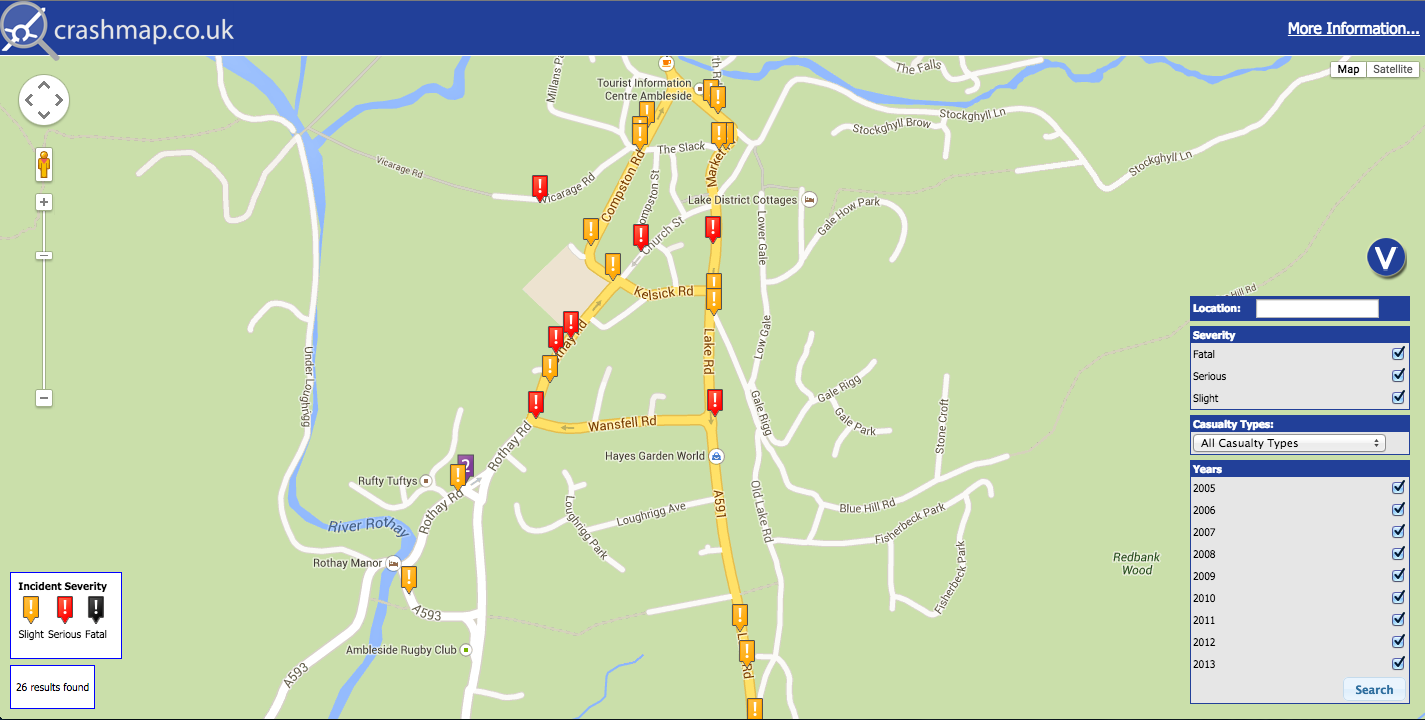
\includegraphics[scale=0.25]{crashmap}
	\caption{Crash Map application}
	\label{fig:crashmap}
\end{figure}

Collision Map \citep{DepartmentforTransport} is similar in purpose to Crash Map. It displays the location of collisions on an interactive map, and also has filters that can be used, including severity, casualty age band and vehicle type (see \autoref{fig:collisionmap}). It differs to Crash Map in that you must select a local highway authority rather than searching for a location or using the map to find it. Clusters of collisions are displayed as one marker on the map, with a number representing how many collisions are in that area. You can reveal the exact location of each collision by zooming in further.

Collision map has several useful features, but has similar limitations to Crash Map. The main advantage of this application is the grouping of collisions to signify hotspots. This makes it very easy to look at an area and see where the most collisions have occurred. A disadvantage in comparison to Crash Map is that it is only possible to use collision data for one year in any search. Like Crash Map, it also lacks the capability of analysing particular routes. This becomes particularly difficult if a route passes through more than one highway authority as the user would need to change the search parameters. 

\begin{figure}
	\center
	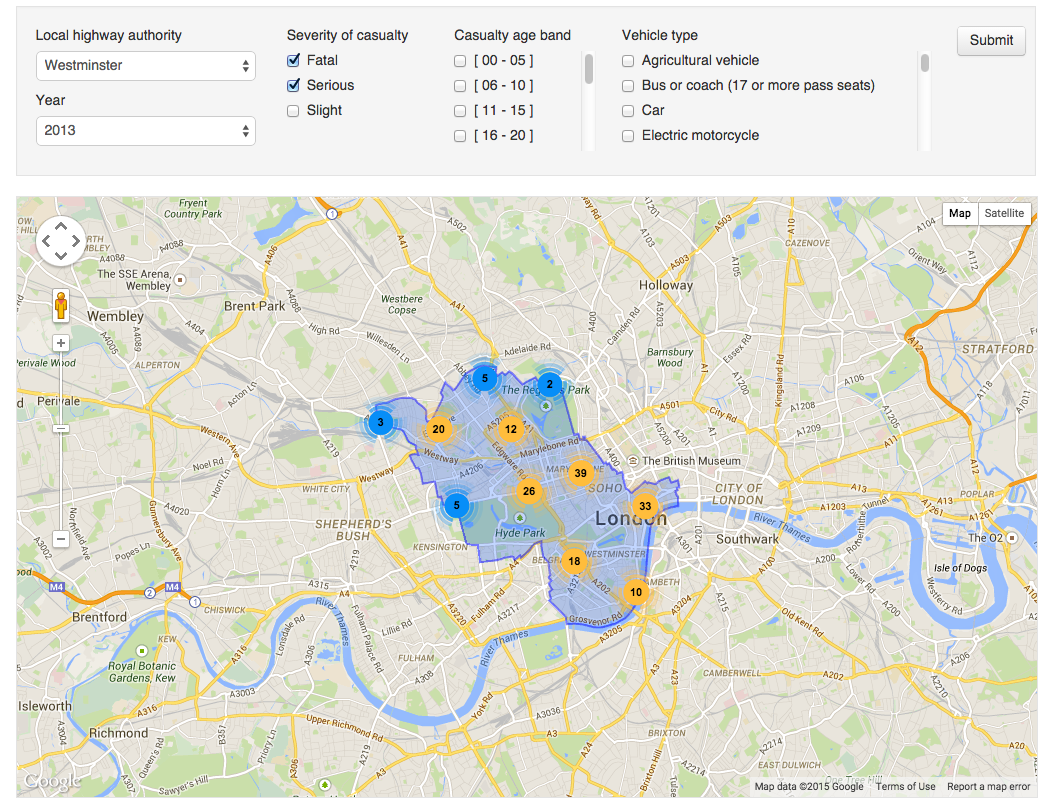
\includegraphics[scale=0.3]{collisionmap}
	\caption{Collision Map application}
	\label{fig:collisionmap}
\end{figure}

Motorcycle Accidents \citep{Mceinsurance} provides an interactive guide to motorcycle collisions in the UK. The aim of this application is to provide motorcyclists with information about where and when it is safest to ride. The application presents statistics about motorcycle collisions filtered by region (see \autoref{fig:motorcycle}). The application makes use of several fields from the Open Datasets, including road conditions, time of day and severity. For each field, it is possible to view a break down of the data in each region. For example, a user can analyse how collisions depend on time of day in London. The application also presents two key facts for each field in order to summarise the data.

The data is presented in a manner that is easy to analyse for any user, and the facts give a concise summary of the findings from the data. This is adequate to serve the application's purpose, but there are limitations that affect the overall usefulness. For example, it is not possible to view specific collision hotspots. The regions cover very large areas, and there is no breakdown of where the collisions occur within these areas.

\begin{figure}
	\center
	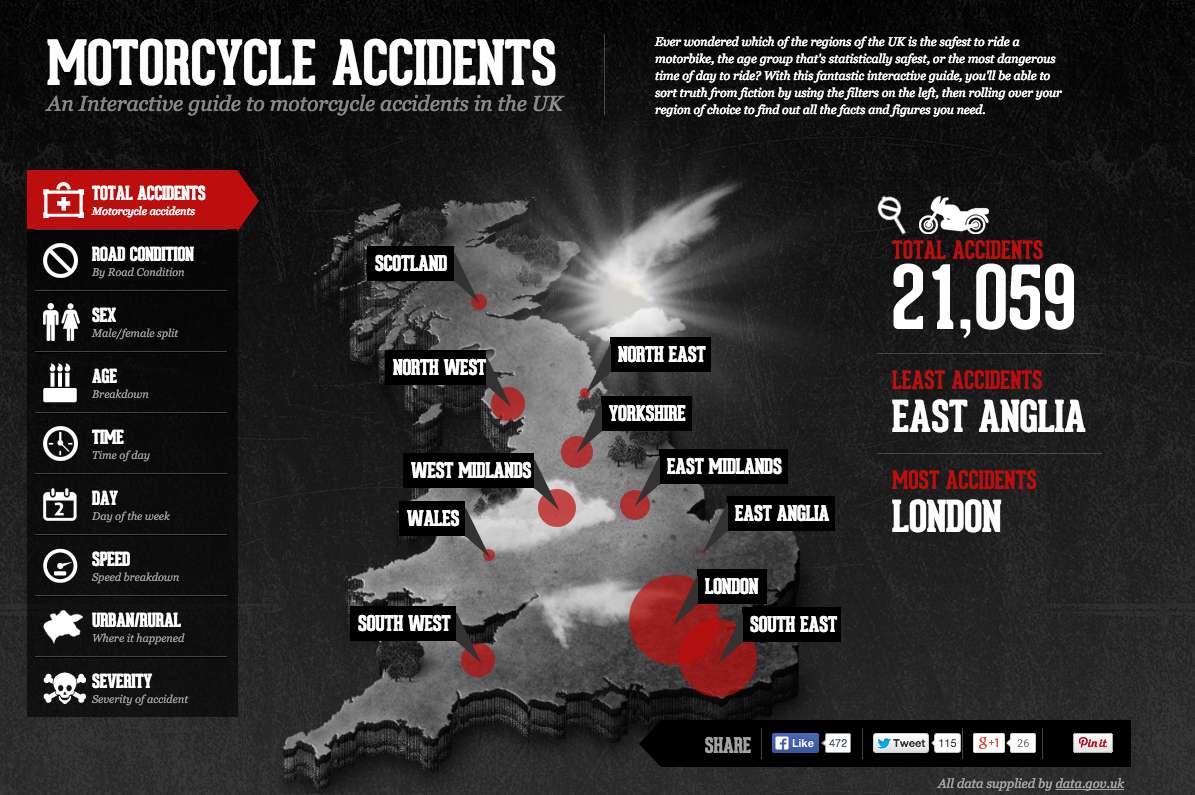
\includegraphics[scale=0.3]{motorcycle}
	\caption{Motorcycle Accidents application}
	\label{fig:motorcycle}
\end{figure}

The final application reviewed for this project is Walkonomics \citep{Davies}. Walkonomics aims to rate the 'walkability' of streets around the world by combining the views of large groups of people, local communities and Open Data. A user can search for a location, and the application will return a list of streets near that location, along with a map displaying markers for each street (see \autoref{fig:walkonomics}). It is then possible to click on a street name in order to find out more information about that street. This page presents a list of reviews for that street, including one from 'Walkobot' which is based on various Open Datasets. Additionally, a user may add a review of their own on this page. 

Walkonomics extends what the other applications have achieved with Open Data. Not only does it use Open Data from different countries, but it also uses different types of data (road safety and crime are mentioned). In addition to this, it combines the use of Open Data with crowdsourcing. Beyond being a web application, Walkonomics is also available to download as an App on both Android and iOS devices.

However, there are some major limitations to this application. For example, when searching for several major cities across the world (including Cardiff, Edinburgh, Paris, Sydney and Los Angeles), no results are found (this behaviour was observed when exploring the application available online on 10/4/2015). It is unclear whether this is a bug or expected behaviour. Additionally, there is no transparency over which Open Datasets are used; it mentions the use of road safety and crime data, but does not specify which countries/states they have obtained this data from. As an application that claims to use data from various different sectors and sources, it should provide a more detailed list of datasets used.

\begin{figure}
	\center
	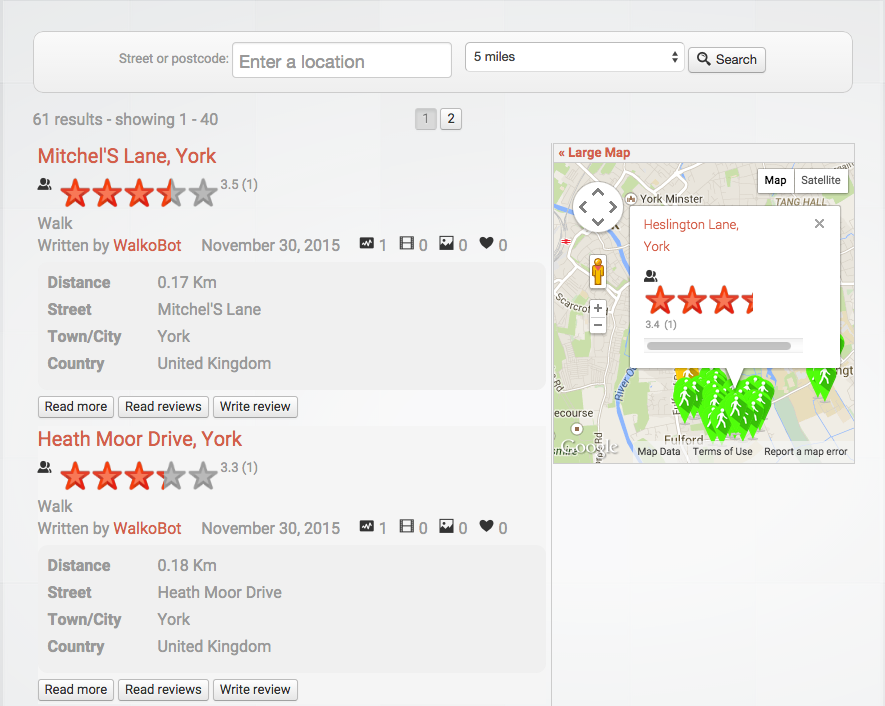
\includegraphics[scale=0.4]{walkonomics}
	\caption{Walkonomics application}
	\label{fig:walkonomics}
\end{figure}

The four applications discussed are compared in \autoref{tab:applications}. The following characteristics were not included in the table as they are common to all four applications:

\begin{enumerate}
  \item The applications are not open source.
  \item The applications are not capable of filtering collisions by route.
\end{enumerate}

\begin{table}[tbp]
	\center
   \caption{Comparison of applications that use road safety data}
  \begin{tabular}{  p{2.2cm}   p{3.0cm} p{2.2cm}  p{2.0cm} p{3.5cm}  }
  	\hline
      \textbf{Application} & \textbf{Data} & \textbf{Platform(s)} & \textbf{Mapping API} & \textbf{Data Filters} \\ \hline
    Crash Map & UK Road Safety 05-13 & Web & Google Maps & Severity, Casualty Types, Year\\ 
	Collision Map & UK Road Safety 05-13 & Web & Google Maps & Highway Authority, Year, Severity, Casualty Age, Vehicle Type\\ 
	Motorcycle Accidents & UK Road Safety 2011 (Motorcycle Only) & Web & N/A & N/A\\ 
	Walkonomics & Road Safety, Crime & Web, iOS, Android & Google Maps & N/A\\ \hline
  \end{tabular}
  \label{tab:applications}
\end{table}

As these applications all rely on Open Data, it is disappointing that the developers have not made their code available. The community would benefit greatly from this, as people looking to build new applications in the field would be able to more thoroughly analyse the existing work. By sharing ideas about how to develop such applications, the community can work together to improve them and agree on the best approach.

Another noticeable aspect from this comparison is the similarity between Crash Map and Collision Map. In fact, there are several other applications listed on \textit{data.gov.uk} that are similar to these. This led to the Department for Transport taking Collision Map offline in March 2015, as they felt it offered low value to taxpayers due to the number of alternatives available.  All of these applications operate in the same way; the user zooms to an area of the map, and all collisions within that area are displayed. There are no advanced searching facilities available, such as searching for collisions on a particular route only. If a user wanted to find such information, they would need to find the route, and manually pan the map, counting how many collisions are plotted. Clearly there is room for a new application that provides more advanced features like this.  


\section{Web Application Development}

\subsection{Overview}

Jazayeri's study of trends in web application development discusses the area of web application development from a software engineering perspective \citep{Jazayeri2007}. The Web is described as "an attractive playground for software engineers where you can quickly release an application to millions of users and receive instant feedback". It is argued that web applications reach "users that are varied in age, culture, language, education, interest, needs, etc.", and that many challenges are raised when providing for such a varied group of users. However, whilst all applications may be able to reach such a varied audience, it could be argued that most have a specific target audience that the application can be catered to. Hence the challenges of providing for a varied user base is more dependent on the type of application, rather than the platform on which the application is available. 

A major benefit of web applications over desktop applications is the ease in which new versions can be released. In a desktop application, even a small bug fix will require a new version to be installed for all clients. This can lead to numerous issues, as explained by Jazayeri \citep{Jazayeri2007}. In contrast, a web application exists on one server and the browser acts as a universal client. This means that features and bug fixes can be deployed immediately, and users will instantly have access to the upgraded application without having to install an update. This leads more kindly to an agile development strategy, as small updates can be released at any time with no impact on users. In contrast, desktop applications are more likely to require updates to be grouped together in order to reduce the number of updates that the user must install. However, it is worth noting that some web applications may also require updates to be bundled if they require downtime in order to be applied.  

Web development has been "driven by a move towards open source and standardised components" \citep{Jazayeri2007}. This trend is seen right through web development, from the application itself to the server that it is hosted on. The standard open source server environment used by many is commonly referred to as LAMP. This represents the operating system (Linux), the web server (Apache), the database server (MySQL), and the scripting language (PHP, Perl or Python). The main advantage of a  LAMP environment is that it can be assembled relatively easily and cheaply. PHP, MySQL and Apache are the three most commonly used tools in their respective categories. They have all been developed by programmers within the community who focus on writing features that they want and need \citep{Nixon2009}. As the code is available for all to see and change bugs can be resolved and potential security issues can be prevented before they happen.


\subsection{Programming Languages for Web Application Development}
\label{webproglanguages}

This section compares and contrasts some of the most popular programming languages used for web applications. The focus is on three of the most popular server-side scripting languages that are used in modern web applications; PHP, Python and Ruby. There is also a discussion of the most popular client-side scripting language, JavaScript.

PHP is a server scripting language designed by Rasmus Lerforf. It is fast, flexible and one of the most popular scripting languages available. According to Netcraft's Web Server Survey of January 2013, PHP was being used by 244M sites at this time \citep{Ide2013}. This equates to 39\% of all sites used in the survey. A large factor behind this popularity is the number of content management systems and ecommerce solutions that are written in PHP; WordPress, Joomla, Drupal, Zencart, osCommerce and Megento account for 32M of these sites. PHP's main advantages include the number of built-in libraries for common web tasks, the ease of learning and use, and its portability \citep{Welling2005}. Its flexible integration with HTML makes client tier integration easy. The main disadvantage of PHP stems from its huge popularity. Because of the huge number of applications authored in PHP, hackers are presented with a "huge and rather attractive attack surface" \citep{Ide2013}. Additionally, due to the open source nature of PHP, it is easier for hackers to find exploits. 

Ruby is a dynamic, imperative, object-oriented programming language developed by Yukihiro Matsumoto. Ruby on Rails is a popular framework for web application development, based on the model view controller pattern. This framework adds a set of powerful functionalities such as "scaffolding, active record, migrations, routing, environments, and many helper functions" \citep{Jazayeri2007}. Advantages of Ruby include better security features, pure object-oriented programming, highly readable code and good testing frameworks. Disadvantages include a steep learning curve and a lack of informational resources.

Python was first released in 1991 by Guido van Rossum. In contrast to PHP, it was initially designed as a full-featured general purpose language. It supports multiple programming paradigms, including object-oriented and functional programming. Its design philosophy emphases code readability. Python is quick and easy to learn and it has a large community who provide good support. Disadvantages of Python include its lack of true multiprocessor support and absence of commercial support. 

A comparison of these three languages is presented in \autoref{tab:weblanguages}. The languages have been ranked based on several criterion, with 1 signifying the best rating and 3 the worst. The rankings are based on previous discussion, further research and Klaus Purer's study \citep{Purer2009}. Purer found PHP to be most popular, followed by Python, with Ruby the least popular. GitHut is an online tool that analyses how popular programming languages are on GitHub \citep{Zapponi2014}. It shows that in Q4 of 2014, Python featured in more active repositories than PHP and Ruby. Whilst this suggests that the relative popularity may have changed since Purer's report of 2009, the TIOBE Index for March 2015 still shows PHP above Python \citep{TIOBESoftware2015}. The next comparison is based on the ease with which the language can be learned ('learnability'). These rankings are based on Purer's discussion on readability, and personal opinion from looking at the languages. The rankings for security are based on Purer's conclusion where he found PHP to be slightly behind the others. PHP is mainly criticised for allowing poor programming practices which "result in many security related bugs". All of these languages are open source, which can raise security issues as hackers can use the source code to identify vulnerabilities before attacking sites. 

\begin{table}[tbp]
	\center
   \caption{Comparison of PHP, Ruby and Python, based on  \citep{Purer2009}}
  \begin{tabular}{l l l l}
  	\hline
      \textbf{Criterion} & \textbf{PHP} & \textbf{Ruby} & \textbf{Python} \\ \hline
      Popularity & 1 & 3 & 2 \\ 
      Learnability & 2 & 3 & 1\\ 
	  Security & 2 & 1 & 1 \\ 
	  Community & 1 & 2 & 1 \\ \hline
  \end{tabular}
  \label{tab:weblanguages}
\end{table}

The following criteria were not included in the table as the languages were considered to be equal for them:

\begin{enumerate}
  \item Performance.
  \item Database abstraction.
  \item Exception handling.
  \item Available frameworks.
\end{enumerate}

Performance of the languages was compared by Purer, and he considered them too similar to differentiate. He argued that PHP was inferior when it comes to database abstraction and exception handling, as these features hadn't been implemented correctly in some long-living PHP projects. This is an unfair conclusion as PHP does include the features. An unbiased comparison of the three languages should focus purely on the features of the languages, rather than the implementation of the features by some developers. All three languages have highly popular web frameworks with thriving communities. Examples include Laravel for PHP, Rails for Ruby and Django for Python.

Client-side JavaScript combines "the scripting ability of a JavaScript interpreter with the Document Object Model (DOM) defined by a web browser" \citep{Flanagan2006a}.This means that it can add behaviour to otherwise static web content. This technology is the core of web development technologies like Ajax (Asynchronous JavaScript and XML). JavaScript helps reduce server usage, as functions that were typically performed on the server can be done on the client (e.g. form validation) \citep{Jazayeri2007}. Browsers are able to provide more responsive operations to the user by pushing some of the client-server communication to the background while the application is still interactive. This can be achieved using Ajax to introduce an intermediary 'engine' between the user and the server \citep{Garrett2005}. Every user action that would normally generate a HTTP request becomes a JavaScript call to the Ajax engine instead. If the engine needs something from the server to respond (e.g. retrieving new data), the engine makes those requests to the server asynchronously without interrupting the user's interaction with the application. 


\subsection{Model-View-Controller}

A large number of contemporary web frameworks make use of the Model-View-Controller (MVC) design pattern. The Model is the application object, the View is its screen representation, and the Controller defines the way the user interface reacts to user input \citep{Gamma1995}. The MVC pattern had been popular in software engineering for many years before it was realised that it could be applied just as well to web applications \citep{Jazayeri2007}.  The main problem with using the MVC design pattern when developing web applications is that the application must be partitioned between the client and the server \citep{Leff2001}.

Morales-Chapar et al. provide an interesting discussion on the different implementations of MVC in web applications \citep{Morales-Chaparro2007}. This paper focuses on "web applications which are data dynamic and typically written in two programming languages", much like the application developed for this project. A case study is used to compare the advantages and disadvantages of server-side MVC with two mixed client-side and server-side MVCs. 

Server-side MVC is derived from desktop MVC, in that all components are usually programmed in the same language and the server runs all computations and operations. It is pointed out by Morales-Chaper et al. that this approach is useful when an "application's capabilities requirements are poor at client side (e.g. mobile browsers without JavaScript functionality) or when application necessity is only to display information with low levels of user interaction". It is worth consideration that this paper was published in 2007, and since this time mobile devices and browsers have advanced significantly, so the first advantage given is of little relevance now. The disadvantages of this approach include the incapability of updating part of a view, increased bandwidth usage and the higher server usage due to the server validating forms, amongst other things.  

The first mixed client-side and server-side MVC discussed by Morales-Chapar et al. was designed with a focus on resolving the previously raised issues. This MVC design involves dividing the Controller and View between the server and client, whilst leaving the model at server-side. In this system, some processing is now done on the client-side; for example, form validation using JavaScript. They raise the issue of different browsers and operating systems causing issues when accessing UI elements. Whilst the situation has improved since 2007, there still exists the issue of browsers not implementing exactly the same standard specifications. This approach still has the disadvantage of not being able to retrieve data asynchronously without refreshing the page. Without a model on the client-side, there are limitations on providing high interaction levels, and data manipulation becomes more difficult. In comparison with the pure server-side approach, there is an increase in computation time and complexity due to the logic now present on client-side. 

The second mixed client-side and server-side MVC discussed by Morales-Chapar et al. is similar to the previous design, but with part of the model on client-side. This design addresses the issue of not being able to retrieve data asynchronously without refreshing the page, by allowing for the use of Ajax. Limitations of this design include slower computation for tasks requiring access to the server, difficulty of designing a client-side model that is compatible with all browsers, and increased overhead on communications among MVC design elements. 


\section{Software Development Methodologies}

This section features a discussion of some popular software engineering methodologies that were considered for this project. The discussion focuses on those that are most beneficial to a project like this one, i.e. a web application developed by one person in a limited time frame. 

Pfleeger and Atlee define software engineering as "an approach that combines computer science (which is made up of theories and computer functions) and the customer (who provides the problem to be solved) to develop a set of tools and techniques to solve problems" \citep{Pfleeger}. Software engineering methodologies are a group of methodologies used during the development of applications. Methodologies give details of "what should be done in each phase of the software development process" \citep{Mnkandla2009}. They do not necessarily give details of how things should be done, allowing for some tuning by those using them. 

Agile software development is a "conceptual framework for undertaking software engineering projects" \citep{ITKnowledgePortal}. Agile methods generally try to minimise risk by developing software in iterations, which typically last one to four weeks. Each iteration of the project is like its own project, featuring its own planning, requirement analysis, design, coding, testing and documentation phases. At the end of each iteration, a new working version of the application should be available. The team is then able to re-evaluate the project priorities ahead of the next iteration. Agile methods emphasise working software as a primary measure of progress.

Scrum is a software-management process for iterative-incremental software development projects. Scrum relies on "self-organisation, with the team deciding what to do while management removes roadblocks" \citep{Faridani2011}. Scrum is focused on frequent intermediate deliveries with working functionality. Alongside this, there are frequent risk and mitigation plans produced by the development team. There are daily 'scrums', where the development team meet up to explain progress, describe upcoming work and raise obstacles. 

Extreme Programming is an iterative and incremental development methodology. Key practices of Extreme Programming include: making a rough plan quickly and refining it as thing become clearer, test driven development, re-factoring code, continuous integration of code, and an on-site customer to clarify requirements and make crucial business decisions \citep{Faridani2011}. 

It is clear that the methodologies described are designed for team projects, rather than an individual project like this one. However, there are useful concepts that can be taken from each of them and applied to this project. It will be advantageous to split development work into increments. This encourages the delivery of a new, functional version of the application at regular intervals. This approach is particularly beneficial if there are issues developing a complex piece of functionality in a later increment, as there will still be a functional version of the application from the previous increment. 


\section{Design of Interactive Applications}

A key aspect of designing a successful web application involves focusing on user interaction. This section includes a discussion of some design principles that will help to develop a user-friendly application. 

Rogers et al. state that interaction design is about "developing interactive products that are easy, effective and pleasurable to use from the users' perspective" \citep{Rogers2011}. They define the process of interaction design as four basic activities: establishing requirements, designing alternatives, prototyping and evaluating. These activities are intended to inform one another and to be repeated. The repetition is necessary as, for example, one may find that new requirements are needed following feedback in the evaluation phase. Cooper et al. explain the concept of goal-directed design as designing and constructing products "in such a way that the people who use them achieve their goals" \citep{Cooper2007}. The users should be "satisfied, effective, and happy". The goal-directed design process is divided into six phases: research, modelling, requirements definition, framework definition, refinement and support. 

Some key design principles from these books and other literature are presented in \autoref{tab:designprinciples}.

\begin{table}[tbp]
	\begin{small}
	\center
   \caption{Interactive Design Principles}
  \begin{tabular}{ p{2.0cm} p{9.0cm}  p{2.5cm} }
  		\hline
      \textbf{Design Principle} & \textbf{Description} & \textbf{Source(s)}\\ \hline
    Usability Goals & There are six goals: effectiveness, efficiency, safety, utility, learnability and memorability. Typically assessed using questions. Developers can ask these questions during design process to be alerted early on about any design problems that they have not considered. It is possible to establish quantifiable criteria for some usability goals. For example; time to complete a task (efficiency) and time to learn a task (learnability).  &  Interaction Design: Beyond Human Computer Interaction \citep{Rogers2011}.\\  
     User experience goals & Cover a range of emotions and felt experiences, both desirable and undesirable. Concerned with how users experience an interactive product from their perspective, rather than assessing how useful a system is from its own perspective. Assessed using questions.  &  Interaction Design: Beyond Human Computer Interaction \citep{Rogers2011}.\\ 
       Personas & Descriptive models of users created based on research. Cooper et al. state that personas "provide us with a precise way of thinking and communicating about how users behave, how they think, what they wish to accomplish, and why". They are not real people, but "based on the behaviours and motivations of real people". Personas are depicted as specific individuals, but they also represent a major user group for the application.  &  About Face 3 : The Essentials of Interaction Design \citep{Cooper2007}, usability.gov \citep{USDepartmentofHealthHumanServices}\\  
       Scenarios & A means of imagining ideal user interaction. Persona-based scenarios are "concise narrative descriptions of one or more personas using a product to achieve specific goals". This lets a designer work with a story describing an ideal experience from the persona's perspective, with a focus on how they think and behave. These scenarios help drive requirement definition.  &  About Face 3 : The Essentials of Interaction Design \citep{Cooper2007}, usability.gov \citep{USDepartmentofHealthHumanServices}\\ 
       Requirement Definition & Requirements specify "what information and capabilities our personas require to accomplish their goals". The requirement definition process consists of five steps: "creating problem and vision statements, brainstorming, identifying persona expectations, constructing context scenarios and identifying requirements". Requirements should be specific and able to be verified during testing. Requirements can be derived systematically from goals. &  About Face 3 : The Essentials of Interaction Design \citep{Cooper2007}, usability.gov \citep{USDepartmentofHealthHumanServices}, Goal-oriented requirements engineering: a guided tour \citep{Lamsweerde2001}\\ \hline
  \end{tabular}
  \end{small}
  \label{tab:designprinciples}
\end{table}

The concepts discussed thus far will help to design a system that offers the functionality required by users. Another important aspect of designing interactive applications involves creating a user interface that that is satisfying to use. To help with this, there are some common design conventions applied to most web applications that can be followed. Lynch and Horton discuss some of these conventions in 'Web Style Guide' \citep{Lynch2009}. The first of these conventions is 'restraint and simplicity'. This involves focusing on critical functions of an application and avoiding all "nice-to-have and easy-to-add features". The critical features should be addressed with a design that is "uncluttered by unnecessary elements". Another key convention involves guiding interaction by making the design self-explanatory. A good design should guide users through the functional elements of a page. Instructions, labels, prompts and design patterns can be used to explain what is expected and how the page works. Feedback is crucial to a well designed application. For example, if an error has occurred, it is important to alert the user with a clear error message explaining why an error has occurred and how the user can resolve it. 

\section{Mapping APIs}

A fundamental objective of this project involves using an interactive map to analyse collision hotspots. This requires the use of a mapping API. This section features an analysis of some of the most popular JavaScript mapping APIs that are available; Google Maps, Bing Maps and OpenLayers.  

Google introduced the first mapping API in 2005. The Google Maps API \citep{Google} enables the overlaying of data on top of tiled map layers from Google Maps. It brings the look and feel of Google Maps, that many internet users are already familiar with, to third-party applications. The API can be used by most websites free of charge, but charges will incur if the site consistently generates high traffic (25,000 map loads per day for 90 consecutive days). Google provide a number of services and libraries that can be used by developers looking for advanced functionality. Services include directions, geocoding and street view. There is a geometry library that provides "utility functions for the computation of geometric data on the surface of the Earth" (e.g. you can determine whether a given point is near a line). The visualisation library includes 'heat map layer' functionality for visualising data intensity at geographical points.

Microsoft's Bing Maps API \citep{Microsoft} is similar in scope to Google's API. Bing Maps also offers a free usage tier, with a limit of 125,000 cumulative billable transactions within any 12-month period. It was released five years after the Google Maps API and is still behind in terms of functionality offered, hence its lower popularity. There is a considerable amount of documentation available online, but it is not structured or presented as well as Google's, making it far more frustrating to use. The core API does not have advanced geometry and visualisation libraries like Google Maps API. However, it is possible to import third party modules that offer some of this functionality (such as heat maps). 

OpenLayers \citep{OpenLayers} is an open source mapping API that was initially released in 2006. It is very flexible and powerful but also complex and large. It has an extensive collection of documentation and samples, some of which can be difficult for beginners to grasp. It has a large developer community behind it who have provided plenty of tips and example uses. OpenLayers does not have its own directions service, making route calculation a difficult task. OpenLayers is far more complex than the alternatives and more suitable for GIS experts. A lot of the extra functionality that it offers is not required for a project like this.

From this analysis, it is clear that Google Maps offers the most benefits to this type of project. It was created first, and has consistently grown to keep ahead of the competition. Detailed documentation is available online, and there is a large community of developers who are willing to provide support. The heat map functionality is useful for visualising the density of collisions, thus highlighting collision hotspots. It is also notable that three of the existing applications analysed use the Google Maps API; demonstrating its popularity in the field.

\section{Summary}
This chapter looked at the background of the Open Data movement, and the benefits and challenges that using Open Data can bring. It analysed four applications that use road safety data to gain an understanding of what has already been achieved in the field, and to form motivation for the requirements of Route Risks. Aspects of web application development and mapping APIs, were discussed and analysed to motivate design decisions made later in the report. Software development methodologies were looked at to help decide on the approach used for this project. Interactive design techniques were researched and discussed in order to ensure that the design of  Route Risks used these methods. The next chapter uses these findings to create personas and scenarios, and to define the functional and non-functional requirements of Route Risks.

\chapter{Problem Analysis}

This chapter analyses the problem presented by the project, with a focus on using the goal-directed design process \citep{Cooper2007}. Personas were created to represent potential users of the application. Scenarios describing how these personas would ideally interact with the application in order to achieve their goals are then presented. Finally, the functional and non-functional requirements of the application are defined and justified, using the scenarios and findings of the literature review as motivation. 

\section{Personas} 

Due to the time constraints specific to this type of project, it was not possible to perform the necessary field-work in order to make 'rigorous' personas. Therefore, 'provisional' personas were created based on available data and the literature \citep{Venkatesh2003} \citep{Davis1986}. It is stated by Cooper et al. that the use of these provisional personas has proven more successful than not using user models at all \citep{Cooper2007}. 

Cooper et al. warn of some potential issues to avoid when creating provisional personas. It is important to avoid focusing on the wrong design target. Even if focusing on the correct target, one must be careful to ensure that key behaviours that could differentiate the product are not missed. It is important to focus on behaviours and motivations rather than demographics.

Three personas have been created and are presented in \autoref{fig:personaA}, \autoref{fig:personaB} and \autoref{fig:personaC}. Aspects of Persona A were based on information provided by West Sussex Council about the process used to improve road safety\citep{WestSussexCountyCouncil}.

\begin{figure}
	\begin{framed}
 		Linda is a member of the transport department in West Sussex County Council. Linda has good IT skills after taking several training courses and she is familiar with road safety data. One of the main objectives in her job is to improve road safety in the county. Due to the limited resources of the council, route improvements must be prioritised by Linda. In order to do this, she uses the council's 'accident location map' to find the number of casualties per kilometre on a route. This is a slow, tedious and error-prone task, as she must manually pan the map to find each collision on the route before clicking on each one to find the details. Linda finds this process frustrating and boring, so often assigns the task to a junior member of staff. She believes that resources could be better spent on other tasks if there was an application that automated the process.
  	\end{framed}
  \caption{Persona A: Linda}
  \label{fig:personaA}
\end{figure}

\begin{figure}
	\begin{framed}
 		John is the owner of a company that delivers food products from manufacturers to supermarkets. John joined the company after graduating from his law and finance degree 12 years ago, before eventually inheriting it from this late father. John considers himself a 'tech enthusiast' and is always looking to innovate how the company complete day-to-day tasks. He has recently become interested in Open Data, and how he can use it to benefit his business. He is curious about using road safety data to find out about collision hotspots, so that his drivers can avoid them. He hopes that this will reduce the risk of late deliveries due to traffic delays caused by collisions, whilst also reducing the risk of one of his drivers being involved in a collision. 	\end{framed}
  \caption{Persona B: John}
  \label{fig:personaB}
\end{figure}

\begin{figure}
	\begin{framed}
 		Bethan has recently completed her A levels at a sixth form college in her home town of Southampton, and is preparing to move away from home to study Chemistry at the University of Manchester. She is anxious about moving so far away from home, but also excited about the opportunities for meeting new people. Bethan has recently passed her driving test, but is a nervous driver due to her lack of experience. She owns a car and is determined to take it with her when she moves to Manchester, but she is concerned about the dangers involved with driving on motorways. Bethan has basic IT skills having used computers regularly throughout her education, but does not have any significant interest in technology.		
 	\end{framed}
  \caption{Persona C: Bethan}
  \label{fig:personaC}
\end{figure}


\section{Scenarios}

Context scenarios are used to "explore, at a high-level, how the product can best serve the needs of the personas" \citep{Cooper2007}. These scenarios are used to imagine an ideal user experience whilst intentionally being broad and relatively shallow in scope. Scenarios are critical "both for designing an interface and for usability testing" \citep{USDepartmentofHealthHumanServices}.

The context scenario presented in \autoref{fig:scenarioA} describes how Linda would use the application. Scenarios B (\autoref{fig:scenarioB}) and C (\autoref{fig:scenarioC}) describe ideal user experiences for John and Bethan, respectively.

\begin{figure}
	\begin{framed}
		The new financial year has recently begun, and the West Sussex County Council have a new budget to allocate to road safety improvements. The council needs to prioritise the most dangerous routes in the county by using publicly available road safety data to see where the most casualties have occurred. Linda did this analysis last year, but the council wants new analysis to be done, making use of the latest data released by the Department for Transport.
		
		Linda accesses an online application for analysing road safety on her work computer. She enters the first route's start location and destination, and chooses to search all collision data for the last 3 years. The application returns the weighted collisions per kilometre for the route. Linda makes a note of this number, and then repeats the process for all routes. She is now able to suggest which routes need safety improvements based on these figures.
  	\end{framed}
  \caption{Scenario A: Linda using the application}
  \label{fig:scenarioA}
\end{figure}

\begin{figure}
	\begin{framed}
 		John's company have recently acquired a lucrative contract to deliver fresh goods to a large supermarket chain. There is a strict deadline for when the food must be delivered each day, with little allowance for delays. In order to minimise risk, John wants his drivers to avoid roads with collision hotspots.
 		
 		John logs in to his laptop and accesses an online application for analysing road safety. He begins by inputting the postcodes for the manufacturer and the supermarket. He then decides to only include collisions from the last two years as he believes older data will be less relevant due to road changes. He decides to include serious and fatal collisions only, as these are likely to cause lengthy delays. After John submits his search, the application displays a map with a visual representation of where collisions have occurred on the route. John notices a collision hotspot on the route, and instructs his drivers to take a minor diversion in order to avoid it.
  	\end{framed}
  \caption{Scenario B: John using the application}
  \label{fig:scenarioB}
\end{figure}

\begin{figure}
	\begin{framed}
		As the time for moving away to university is drawing near, Bethan is becoming increasingly nervous about driving a long distance journey for the first time. She has never driven on a motorway before, and is worried about the risks involved. Before leaving, Bethan decides to plan her route using her iPad. She wants to find out about which sections of the journey are the most dangerous, so that she can avoid them. Whilst searching online, she finds an application that serves this purpose.
		Bethan enters her home address and university address into the application, and selects to include collisions from the latest year only as she wants results for the most up-to-date roads. The application provides a visual representation of where the most dangerous sections of the route are. Bethan uses this information to plan a safer route which avoids the most dangerous roads.
  	\end{framed}
  \caption{Scenario C: Bethan using the application}
  \label{fig:scenarioC}
\end{figure}

\section{Requirement Definition}

Requirements can now be derived based on project objectives, findings of the literature review, personas and scenarios, software engineering best practices and software quality standards. The requirements will specify \textit{what} the application should do, and the design chapter will focus on \textit{how} this can be achieved.

\subsection{Functional Requirements}
\label{sect:functReqs}

The functional requirements of the system are presented in \autoref{tab:FunctionalReqs}. The requirements have been ranked by importance to help prioritise them during the development phase. A brief justification of each requirement will now follow. 

The project objectives make FR1 an absolute necessity, as using this data is fundamental to the project. The analysis of existing applications in the literature review led to the formation of FR2. This also addresses the project objective of ensuring that the application implements a new method for analysing the road safety data. Additionally, the context scenarios have demonstrated the need for this functionality for three different types of users. 

Scenario A raises the need for consecutive searches (FR3) and collision statistics as mentioned in FR6 and FR9. The need for additional data filters, as described in FR7 and FR8, is justified by each of the scenarios. It is also notable that two of the existing applications analysed included these filters. 

FR4 addresses the project objective of highlighting collision hotspots, and also satisfies the user goals described in Scenarios B and C. This requirement resembles functionality from some of the applications analysed in the literature review, as it specifies the need for an interactive map.

FR5 focuses on making the interface of the application compact and minimising the amount of effort required from the user. This was advised in the literature regarding interactive design, and also a common feature of existing applications.

\begin{table}[tbp]
\center
\caption{Functional Requirements}
\begin{tabular}{| p{1.5cm} | p{9.5cm} | p{2cm} |}
	\hline
	\textbf{ID} & \textbf{Description} & \textbf{Importance} \\ \hline
	FR1 & The application should use road safety data published by the UK Department for Transport. & High \\ \hline
	FR2 & The application should find a route between two user-entered locations and find collisions on this route. & High \\ \hline
	FR3 & The user should be able to immediately submit a new search after a previous search has finished. & High \\ \hline
	FR4 & Collision density should be represented visually on an interactive map in order to highlight hotspots. & High \\ \hline
	FR5 & The input fields and results should be presented on the same page. & High \\ \hline
	FR6 & The application should calculate and present some statistics using data from the 'accidents' dataset, such as number of collisions, number of casualties, collisions per kilometre, weighted collisions per kilometre and casualties per kilometre. & High \\ \hline
	FR7 & Users should be able to filter collisions included in results by year. & Medium \\ \hline
	FR8 & Users should be able to filter collisions included in results by severity. & Medium \\ \hline
	FR9 & The application should calculate and present some statistics using data from the 'casualties' dataset, such as 'weighted casualties per kilometre'. & Low \\ \hline
\end{tabular}
\label{tab:FunctionalReqs}
\end{table}

\subsection{Non-functional Requirements}

The non-functional requirements of the system are presented in \autoref{tab:NonFunctionalReqs}. These requirements have also been ranked by importance. A brief justification of each requirement will now follow. 

These requirements were derived using the software quality standards, ISO/IEC 9126-1\citep{InternationalOrganizationForStandardizationIso2001} and ISO/IEC 25010:2011 \citep{InternationalOrganizationForStandardizationIso2011}. These standards identify several quality characteristics and subcharacteristics that can be used to evaluate software. The six main quality characteristics specified in ISO 9126 are: functionality, reliability, usability, efficiency, maintainability and portability. The newer standard, ISO 25010, adds security and compatibility to this list of main quality characteristics, whilst also redefining some of the others.

Both NFR1 and NFR7 address the compatibility characteristic. NFR2, NFR3 and NFR5 are all usability/operability related requirements. NFR4 relates to the performance efficiency quality characteristic. Finally, NFR6 focuses on the maintainability quality characteristic.

\begin{table}[tbp]
\center
\caption{Non-functional Requirements}
\begin{tabular}{| p{1.5cm} | p{9.5cm} | p{2cm} |}
	\hline
	\textbf{ID} & \textbf{Description} & \textbf{Importance} \\ \hline
	NFR1 & The application should be compatible with the latest (desktop) versions of Google Chrome, Mozilla Firefox and Internet Explorer. & High \\ \hline
	NFR2 & Users should be able to understand how to use the application without external assistance. & High \\ \hline
	NFR3 & Results of data analysis must be presented in a user-friendly manner. & High \\ \hline
	NFR4 & The data analysis should be scalable, with response times never exceeding 10 seconds for any route within Great Britain. & High \\ \hline
	NFR5 & The system's progress should be displayed whilst data analysis is being performed. & High \\ \hline
	NFR6 & The data model should allow for new datasets to be added in the future. & Medium \\ \hline
	NFR7 & The application should be compatible with tablets and smartphones. & Medium \\ \hline
\end{tabular}
\label{tab:NonFunctionalReqs}
\end{table}

\section{Summary}
This chapter defined three different users of the road safety advisory system, and their motivations for using the application. Scenarios were then presented, describing ideal user experiences for each persona. Based on these scenarios, objectives of the project, and findings of the literature review, the functional requirements of Route Risks were defined. Non-functional requirements were also defined using software quality standards. The next chapter uses these requirements to design Route Risks.

\chapter{Design}

\section{System Architecture}

The high-level architecture of the Route Risks application is presented in \autoref{fig:componentdiagram}.

The Request Handler at the core of the application provides the 'Collision Search' interface that clients can use to request information about collisions on a specified route. This component assembles responses to client requests by using the other components of the application as follows.

The Request Parser provides an interface for extracting the relevant information from a user's request. In particular, this will focus on getting the route start and end locations (FR2), the selected years (FR7) and severity levels (FR8).

The Response Generator is responsible for producing collision statistics (FR6 and FR9) and a visual representation of collision hotspots (FR4) using the results of the collision query generated by the Collision Query Engine. The Mapping API's 'Generate Visual Output' interface is required to create the visual representation of collision hotspots.

The Collision Query Engine is responsible for finding all collisions on the route specified by the user (FR2). The Route Query Engine's 'Find Route' interface is used to get the route for the user's request. This route is then used to search the Collision Database using the 'Get Collisions' interface. This search must also use the selected years and severity levels from the user's request. Finally, the Mapping API's 'Filter Collisions' interface is used to refine the collisions found. 

The Route Query Engine takes the user's specified route and gets the directions using the Mapping API's 'Get Directions' interface.

The Mapping API needs to provide interfaces for: finding the route between two locations, filtering collisions to only include those close to the route (FR2), and generating a visual output that represents collision density (FR4). The decision on which third-party mapping API to use during the implementation was based on the need for these interfaces.

\begin{figure}
	\center
	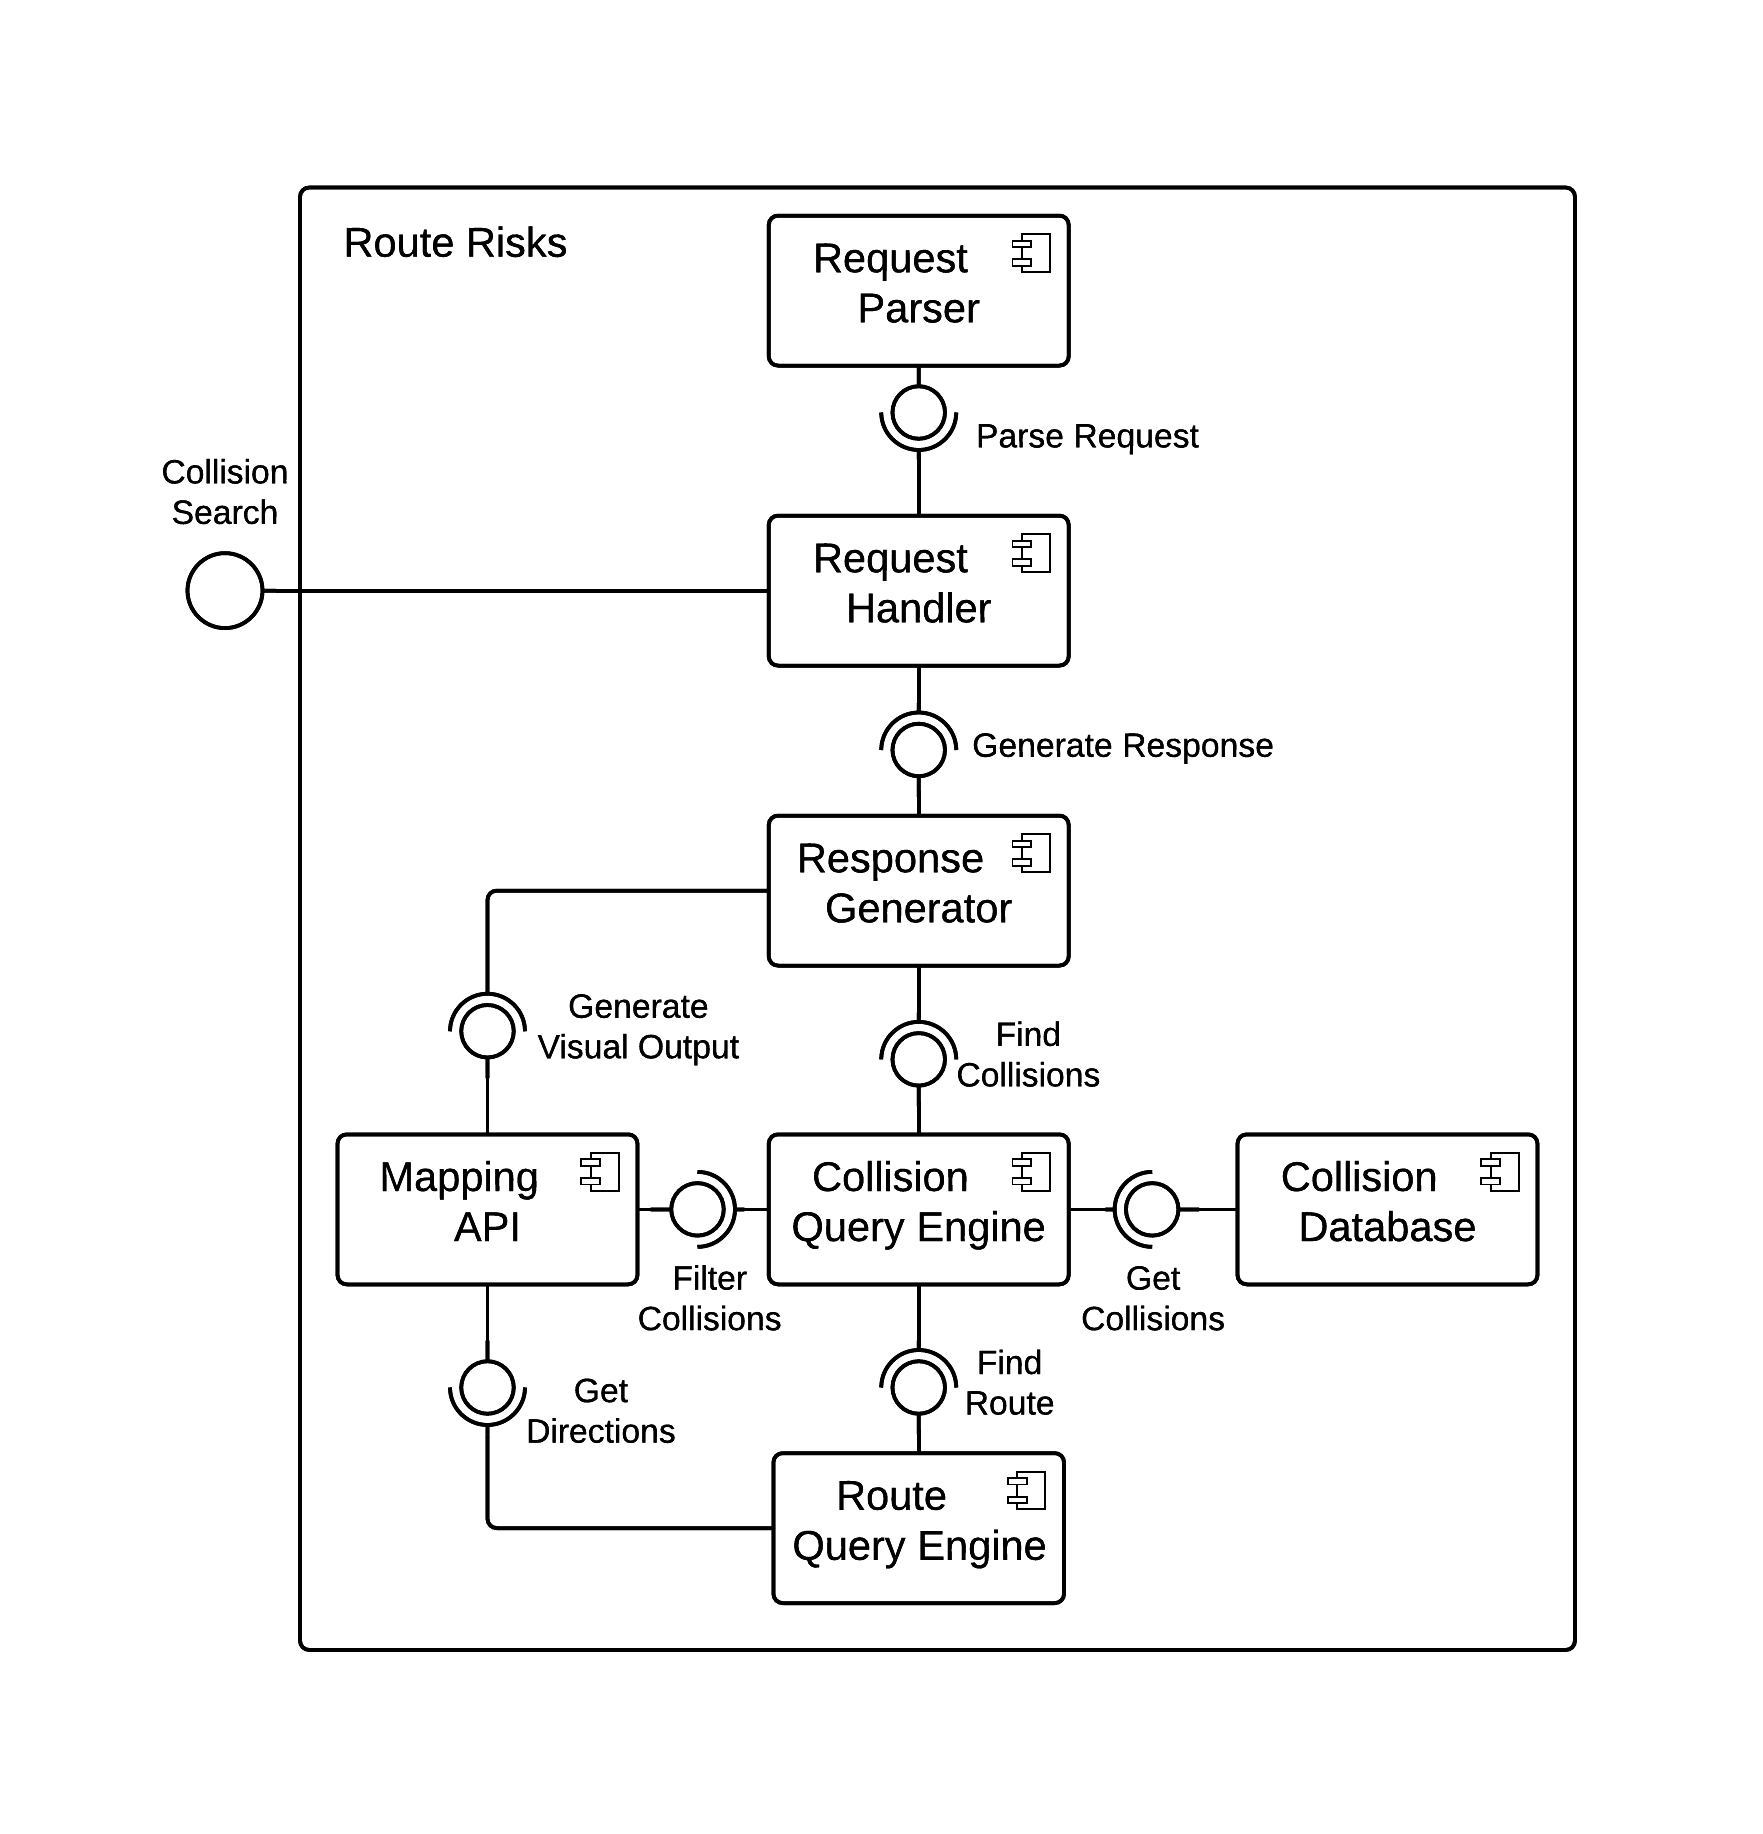
\includegraphics[scale=1]{componentdiagram}
	\caption{Component diagram for Route Risks}
	\label{fig:componentdiagram}
\end{figure}

\section{Request Handling}

The activity diagram in \autoref{fig:activitydiagram} depicts the operations carried out to handle a user request for details about collisions on a specified route. The diagram is partitioned into five sections in order to represent where each of the activities take place. These sections include: the user's view of the application, the user's web browser, the road safety advisory system's application and database servers, and the mapping service. The activities are defined as follows:

\begin{enumerate}
	\item \textbf{Submit search} - The user enters their parameters and submits a search.
	\item \textbf{Validate user request} - Validation tests are run for the user's search parameters.
	\item \textbf{Submit directions request} - If the user's search is valid, the locations entered are submitted to the Mapping Service in order to find a route.
	\item \textbf{Get directions} - The Mapping Service receives the request and attempts to find a route for the provided locations.
	\item \textbf{Send response} - The results of the previous step are used to form a response, before sending it back to the user's browser.
	\item \textbf{Receive directions response} - The response from the Mapping Service is received and checked.
	\item \textbf{Submit collision search} - If a route was found, the response data is processed to get the required data for a collision search. A request is then submitted to the road safety advisory system's application server.
	\item \textbf{Submit database query} -  The application server receives the request, processes the data, and creates a query which is submitted to the database server.
	\item \textbf{Execute database query} - The database server receives the request, and executes the query on the road safety data.
	\item \textbf{Return query results} - The database server sends the query results to the application server.
	\item \textbf{Return collisions} - The application server processes the data received from the database server and sends a response to the user's browser.
	\item \textbf{Filter collisions} - The collisions returned are filtered to exclude those that are too far away from the route.
	\item \textbf{Generate output} - Statistics for the collisions are calculated and the visual representation of collision hotspots is generated. The web page is dynamically updated to display the results.
	\item \textbf{Receive results} - The user sees the results on the page.
	\item \textbf{Error message} - The user sees an error message because their request failed validation, or a route was not found.
\end{enumerate}

\begin{figure}
	\center
	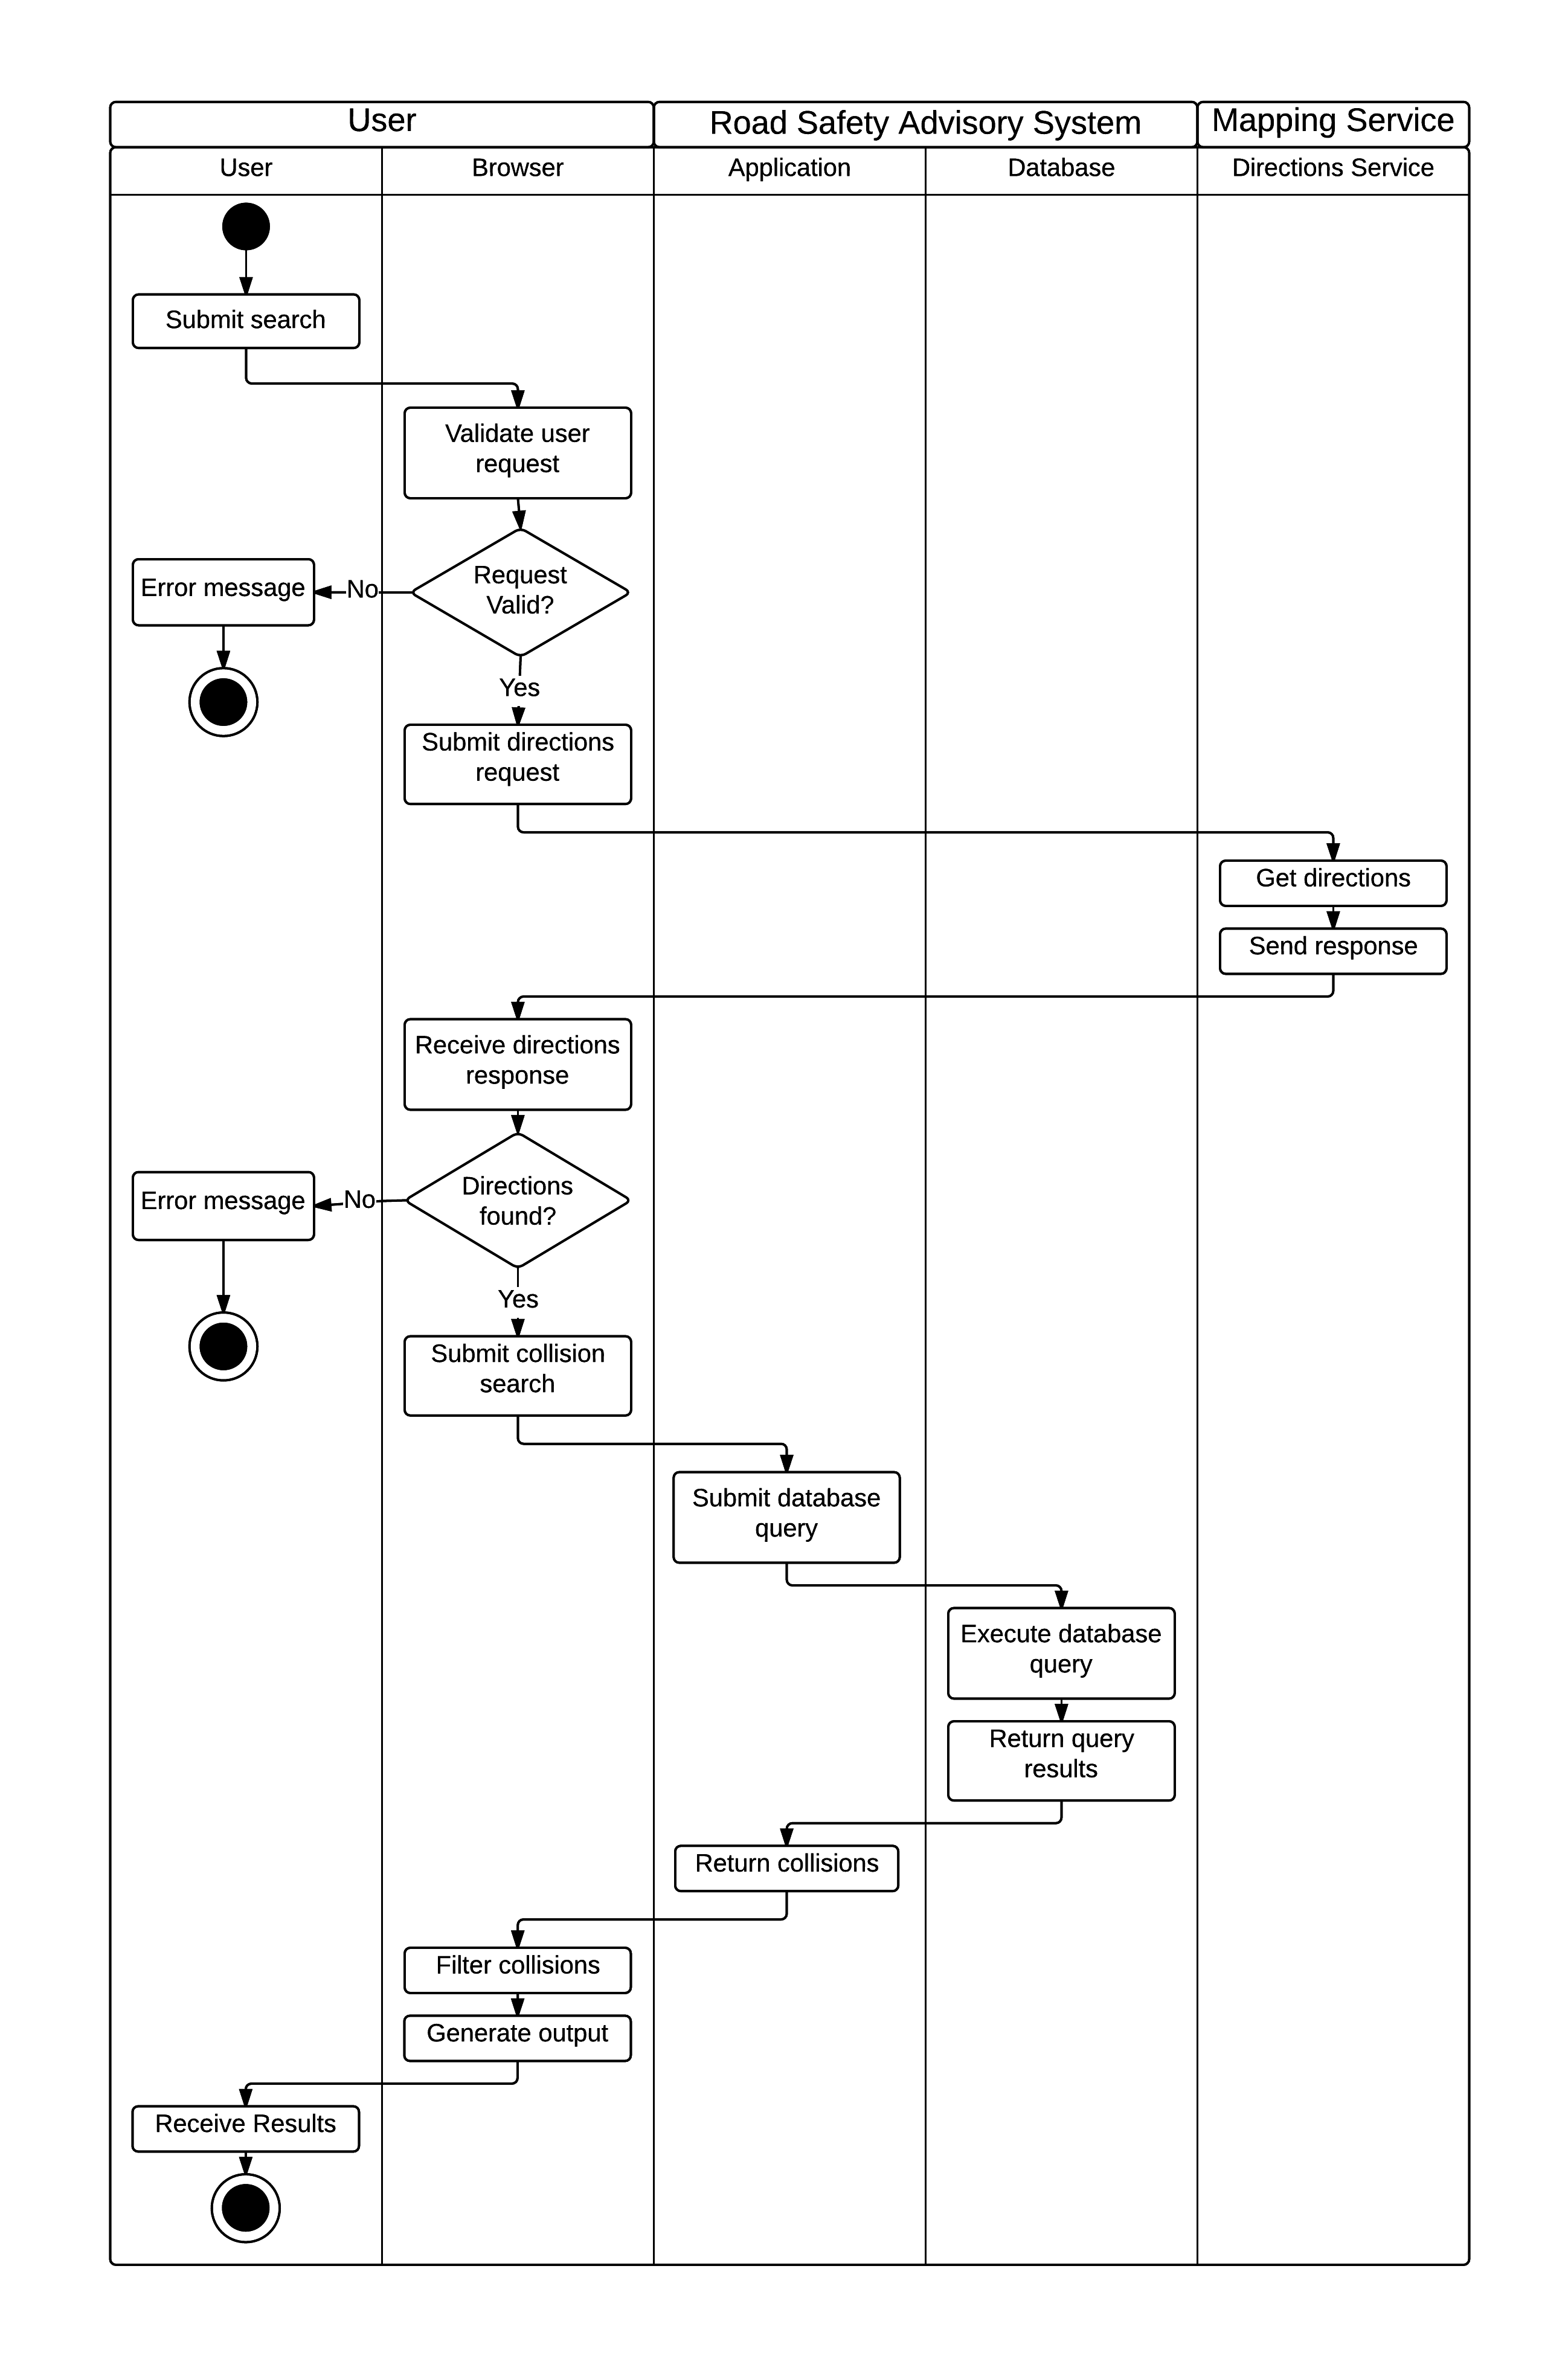
\includegraphics[scale=0.65]{activitydiagram}
	\caption{Activity diagram demonstrating request handling in Route Risks}
	\label{fig:activitydiagram}
\end{figure}

\section{Interface Design}

As discussed in the literature review, the design of a successful web application must focus on user interaction. It is important to follow common design conventions when creating the user interface for a web application, such as those mentioned by Lynch and Horton \citep{Lynch2009}. This section discusses the design of the interface for Route Risks, with justifications for each design decision made. All wireframes presented in this section were created using Lucidchart \citep{LucidSoftware}.

The wireframe for the home page of the application can be seen in \autoref{fig:homewireframe}. The menu at the top of the page includes the site name and links to the pages of the website; Home and About. The decision was made to include the application itself on the home page as users are likely to expect immediate access to it. There is a brief notice at the top of the page explaining how to operate the application in case it is not immediately obvious to a user. A more detailed description of the application is included on the 'About' page in order to keep the home page as uncluttered as possible. 

The main area of the page is split between search parameters and results. These are displayed alongside each other, with 25\% of the width used for parameters and 75\% for results. The results are allocated a larger section of the page as they are the main focus of the application. This creates a visual hierarchy whereby the results, and in particularly the interactive map, will dominate the interface. Displaying the empty results table and blank map on the home page is an example of feedforward, as it helps a user understand what will happen when they submit a search. A user who has never used the application before will immediately expect the statistics in the table to be calculated, and for some representation of the results to be displayed on the map. 

All search parameters are presented in a panel on the left-hand side of the page. The location text fields are displayed at the top, as this is the key information required from the user in order to perform a search. Sample text is included in the field to make it clear that the user should be entering an address. Collision data is filtered by severity and year by using checkboxes. All severity levels and the last 3 years are checked by default. This is a design decision aimed at saving users time, as it is believed that most users will not be interested in data from more than 3 years ago. The submit button is blue in order to draw attention to it and signify that is the primary action on the page.

\begin{figure}
	\center
	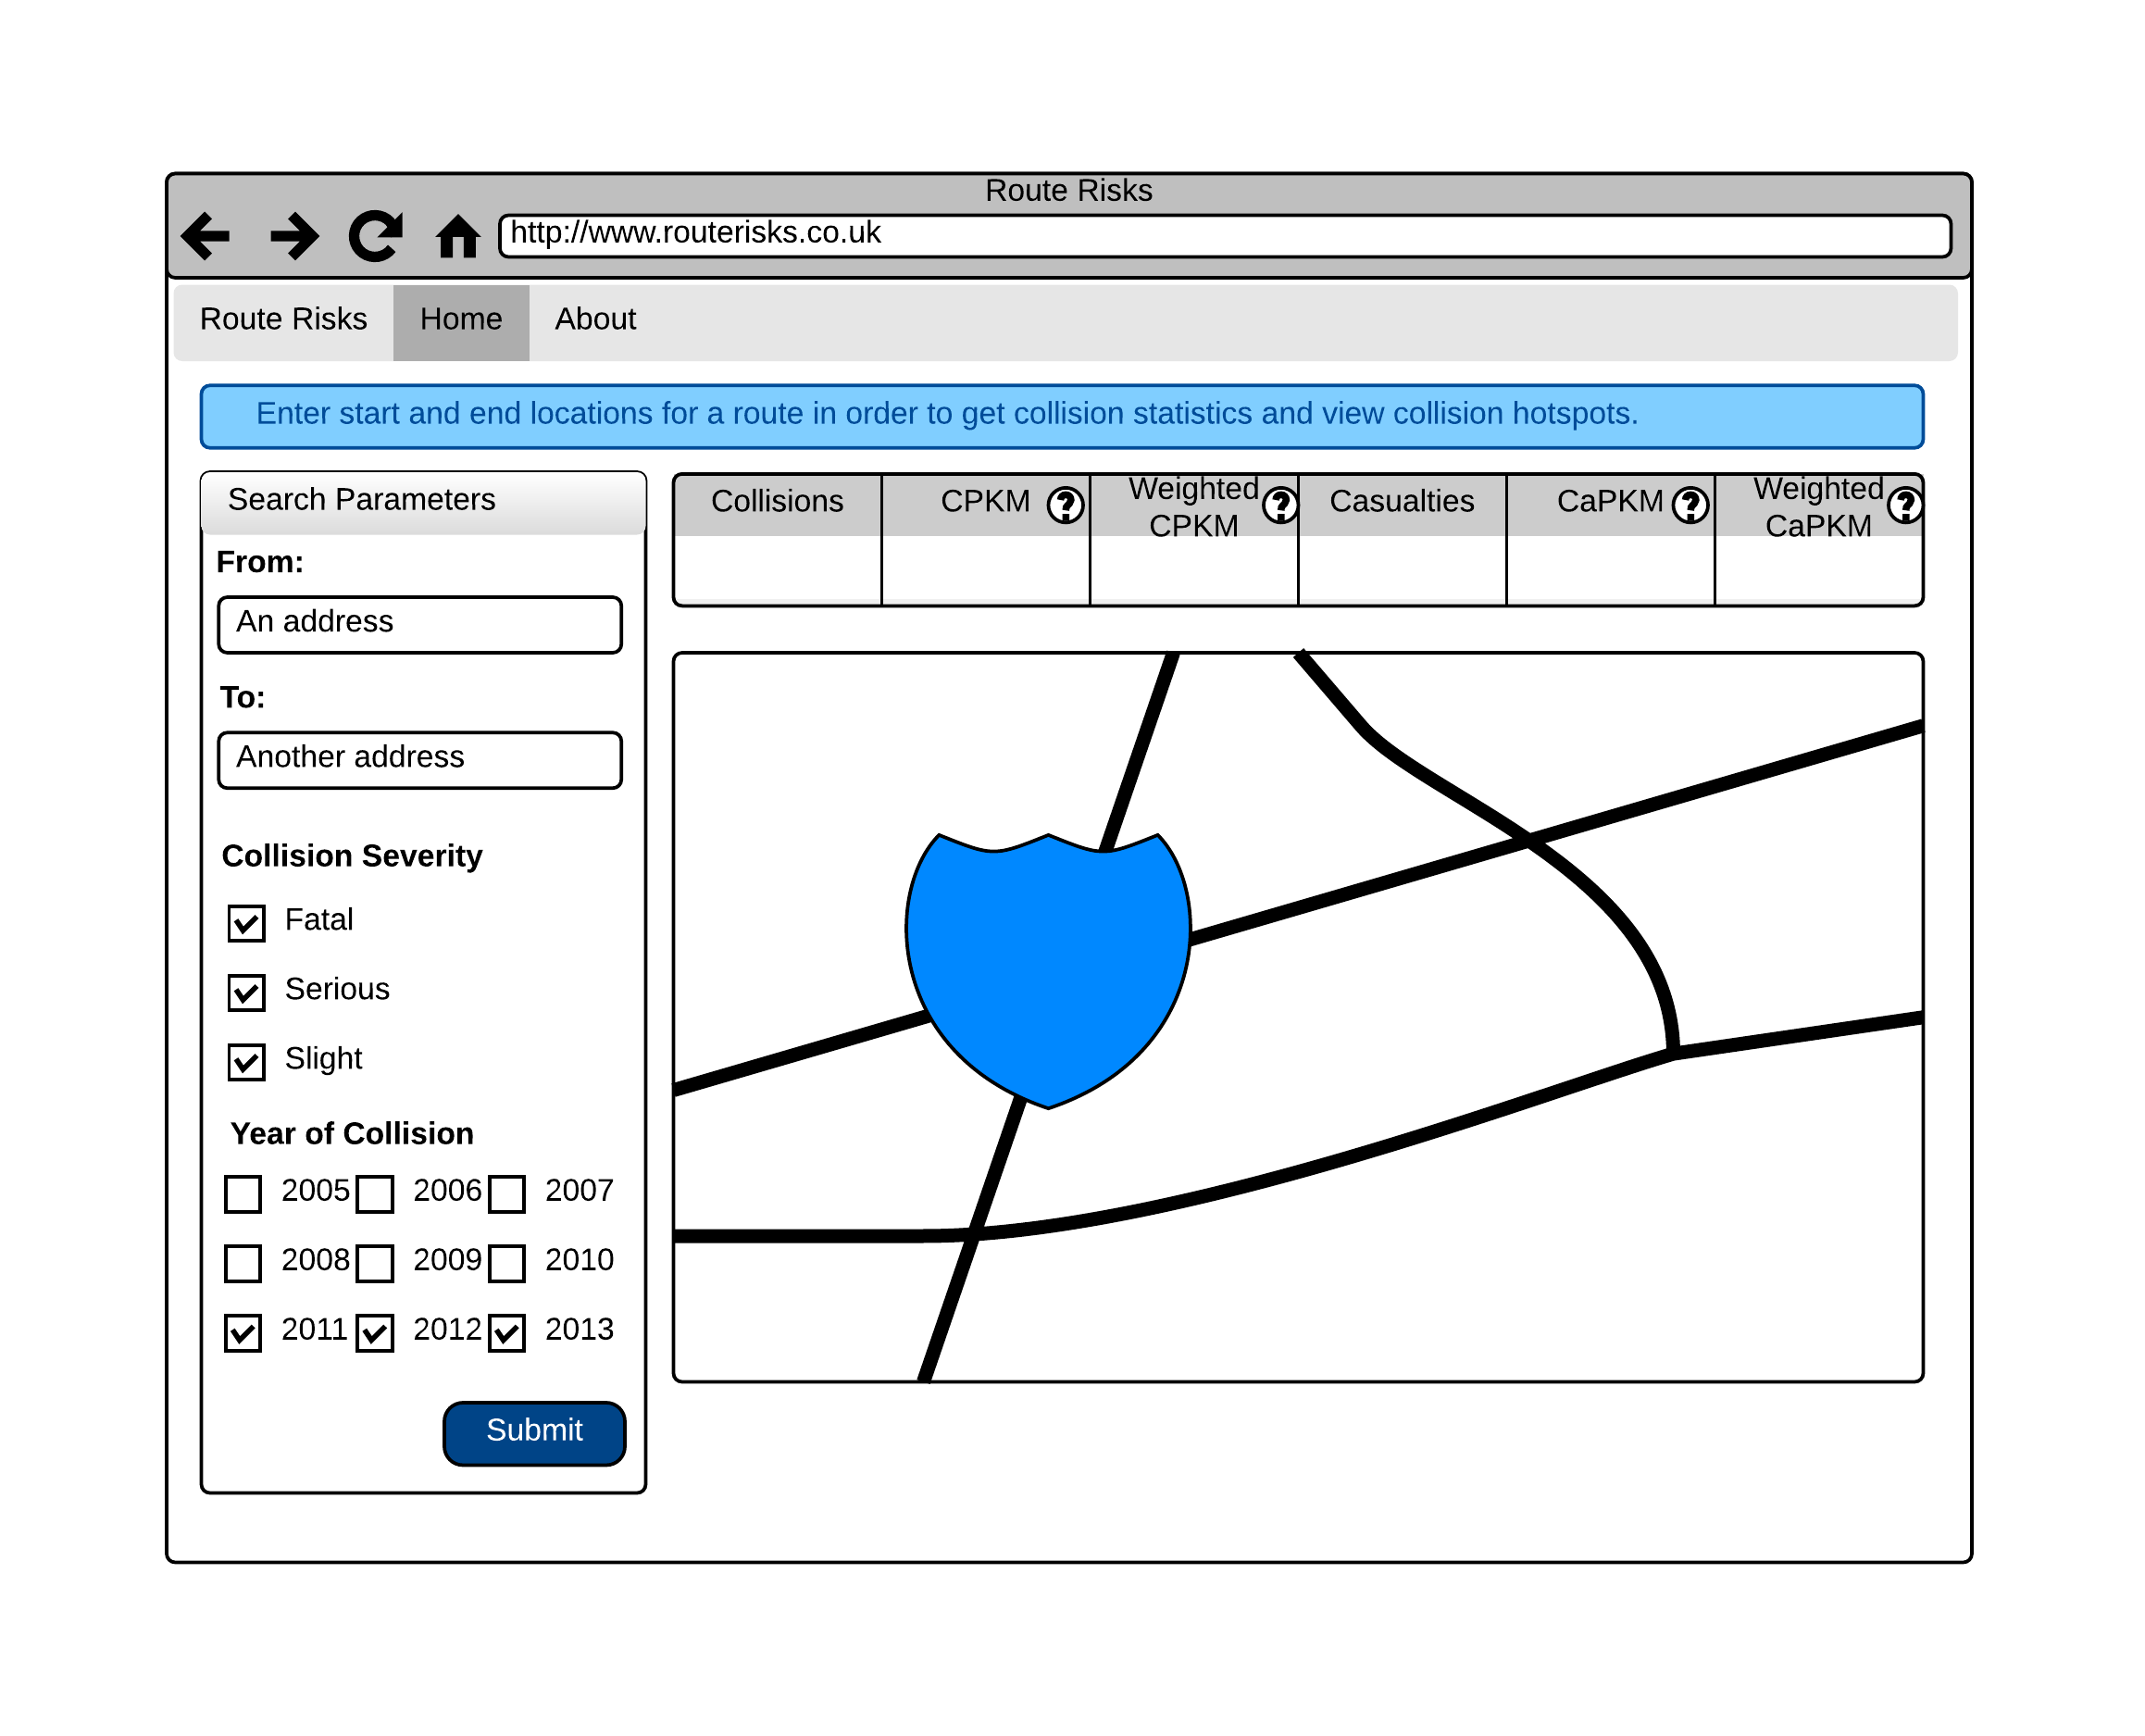
\includegraphics[scale=0.8]{HomePageWireframe}
	\caption{Wireframe for Route Risks home page}
	\label{fig:homewireframe}
\end{figure}

Some statistic names are abbreviated as they are quite long and would make the table look cluttered and text-heavy. These abbreviations will be unfamiliar to new users, so help text is provided by hovering the cursor over the question mark symbol by the corresponding name. A 'popover' is displayed, explaining the abbreviation whilst also providing details about how the value is calculated. An example of this can be seen in \autoref{fig:resultswireframe}.This wireframe shows the application display after a search has completed. The help message at the top of the page is removed as it is no longer required for a user if they have already completed a search. The overall structure of the page remains consistent so that the user is able to submit a new search without complications.

\begin{figure}
	\center
	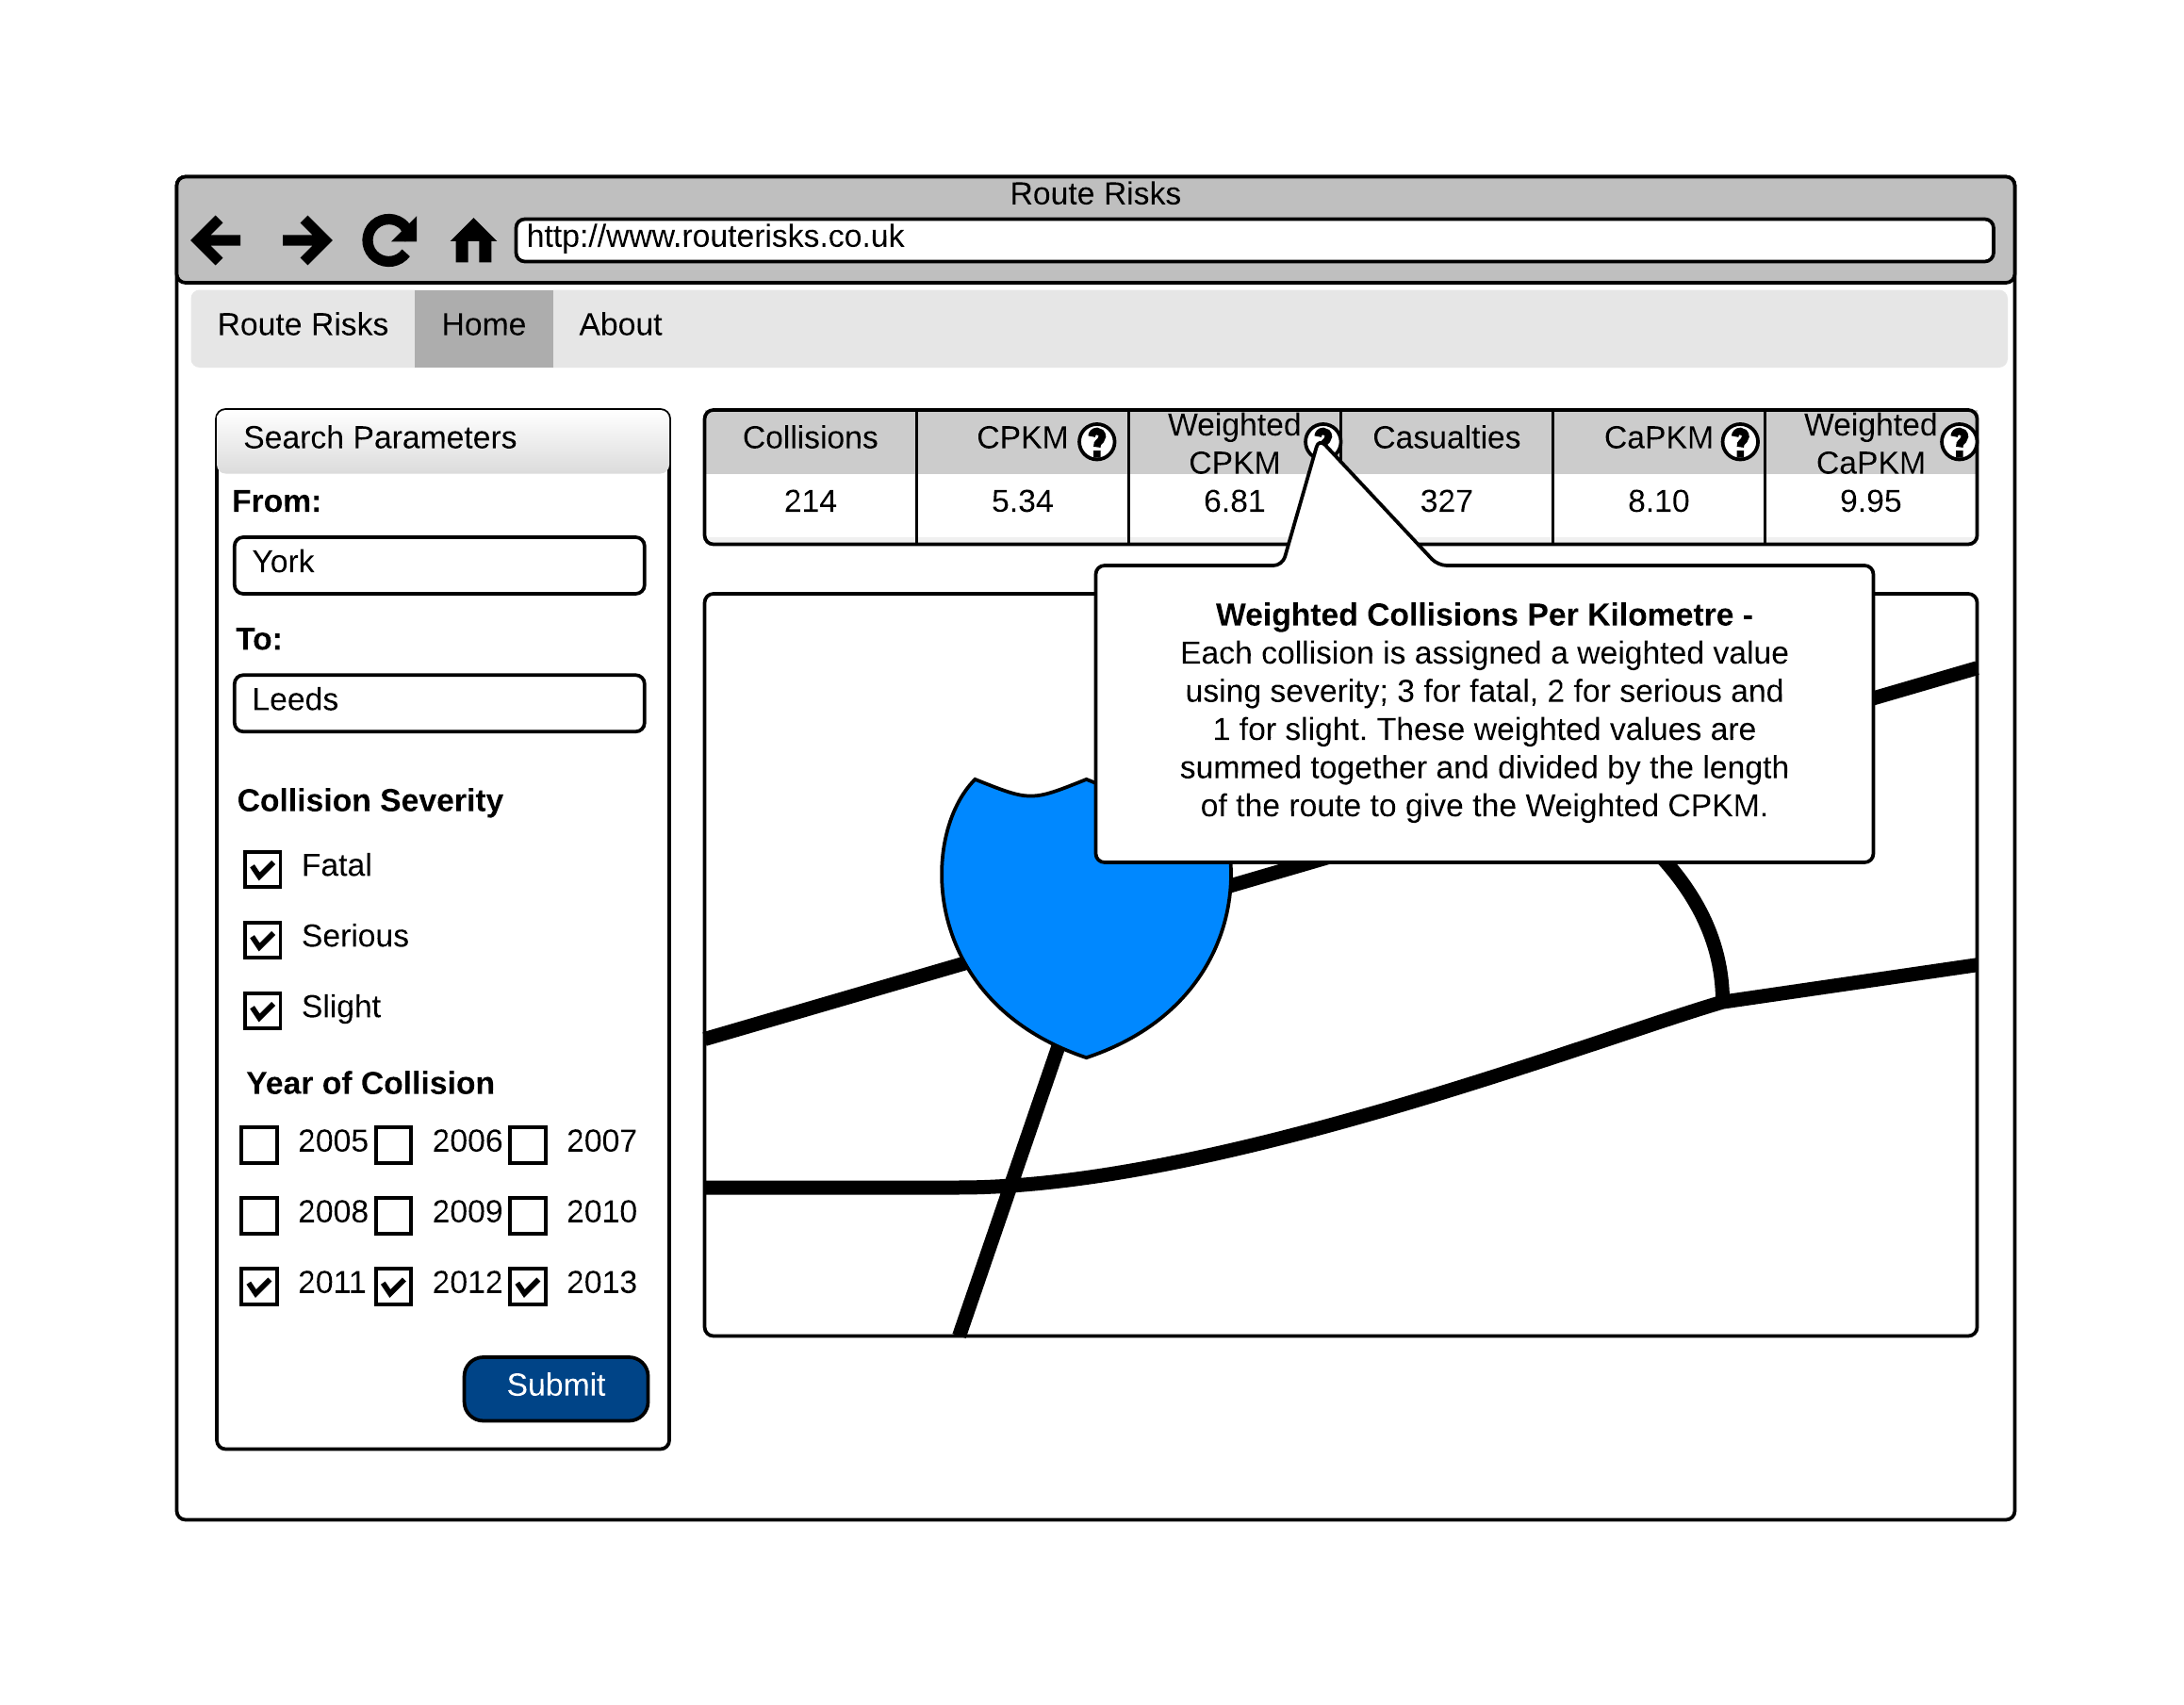
\includegraphics[scale=0.8]{ResultsWireframe}
	\caption{Wireframe for displaying search results}
	\label{fig:resultswireframe}
\end{figure}

The final key design issue involves displaying error messages for the user. If a user submits an invalid request (e.g. submitting a search with all severity levels unchecked), the search will fail and they must be notified. It is crucial that the message is clearly visible and explains what the user did wrong so that they can correct their mistake. An example error message is shown in \autoref{fig:errorwireframe}. The message is displayed in red at the top of the page to grab the user's attention. Red is used as it is commonly associated with errors and warnings.

\begin{figure}
	\center
	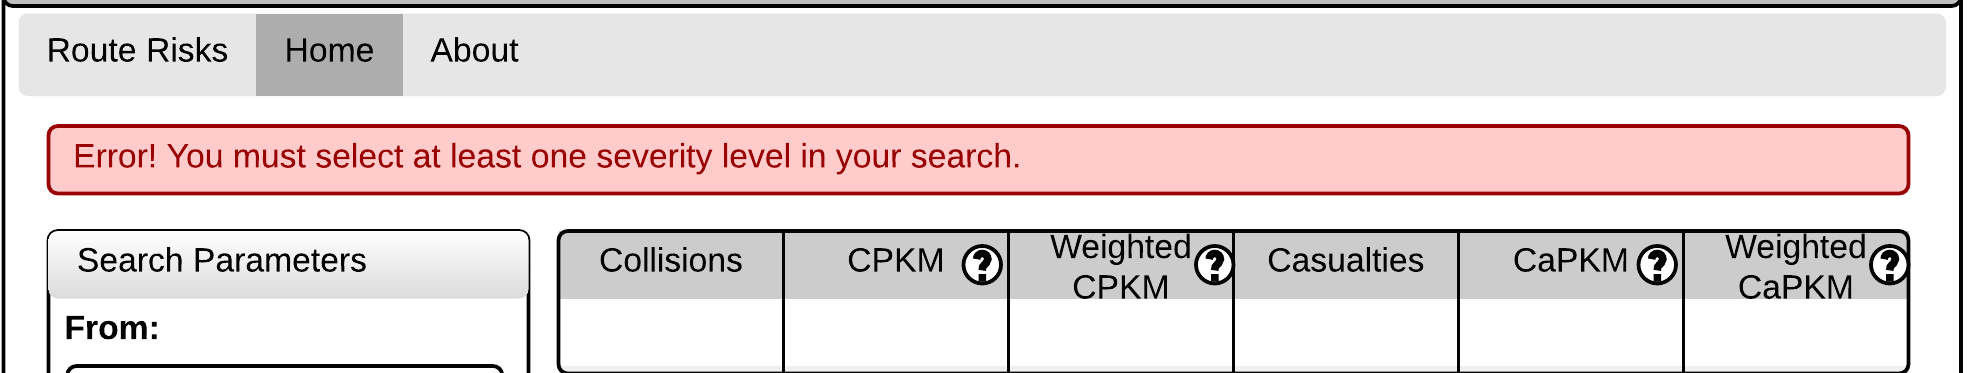
\includegraphics[scale=0.8]{ErrorWireframe}
	\caption{Wireframe for displaying error messages}
	\label{fig:errorwireframe}
\end{figure}

\section{Summary}

This chapter discussed the design of the road safety advisory system. A component diagram is used to represent the high-level architecture of the system. An activity diagram was created to demonstrate the flow of control when handling requests within the system. Designs for the user interface were presented and discussed. The next chapter focuses on the implementation of the system designed in this chapter.

\chapter{Implementation}

\section{Technology Overview}

This section of the report provides a brief discussion of the technologies used in this project, with a justification of why they were chosen ahead of the alternatives available.

\subsection{Google Maps API}

The Google Maps API \citep{Google} was compared with Bing Maps and OpenLayers in the literature review. The findings suggested that Google Maps would be the ideal mapping API for this project. This section justifies the decision made by explaining how the Google Maps API provides the interfaces specified in the design.

The Google Maps API features a Directions Service that receives direction requests and returns computed results. The response contains all relevant information about the route, including distance, duration, an overview path, and latitude/longitude coordinates along the route. This response can be handled by the developer or directly rendered on the map. Route origins and destinations may be entered as text strings or as latitude/longitude values. 

The API's Geometry library contains a function for computing whether a given point lies on or near to a polyline, within a specified tolerance. This function is used to check if collisions are on the polyline returned from the Directions Service. As discussed in the literature review, the API has a visualisation library that lets you create heatmaps. Heatmaps use colour and shape to represent the distribution of data. This is used to highlight collision hotspots, as areas with a high density of collisions are coloured red.

\subsection{PHP}

The evaluation of server-side scripting languages in the literature review pointed towards Python as the favourable option. However, the comparison in \autoref{webproglanguages} only ranks PHP below python for learnability and security. Learnabilty of PHP is not an issue due to the student's familiarity with the language. Security is not a major concern either, as the application does not contain any personal data or passwords (although the correct steps must still be taken to protect the application from malicious attacks). Time constraints on the project make it preferable to use a familiar language rather than learning a new one, so the decision to use PHP was made.

PHP has a large number of popular frameworks (e.g. Laravel \citep{Laravel}, CodeIgniter \citep{codeIgniter} and Symfony \citep{SensioLabs}) that can help to develop projects faster by reusing components and modules. These frameworks also facilitate scalability and long-term maintenance by complying with development standards. Most functionality required by the application is carried out on client-side using JavaScript, meaning that the server-side only needs to create dynamic pages and make some simple database calls. 

Many of the frameworks available are complex and would require a lot of time to be spent reading documentation before implementing simple functionality. Hence the decision was made to use MINI 1\citep{mini}, an extremely simple 'barebone' framework. An exploration of MINI 1's capabilities carried out by this project indicated that it has a very clean MVC structure, PDO for database requests and it uses only native PHP code. It also provides example Ajax and database calls, meaning that most code required for the server-side of the application was easily written by adapting these examples.

\subsection{MySQL}

A fundamental objective of the application involves the use of road safety data published by the UK Department for Transport. This data is published in the comma-separated value (CSV) format. The data must be imported into a database management system so that the application can perform searches on it.

MySQL is a very fast, robust, relational database management system \citep{Welling2005}. The MySQL server controls access to data, enables concurrent access, makes access fast, and ensures that only authorised users are granted access. It uses Structured Query Language (SQL) to query data. MySQL is available under an open source license. Crucially for this project, it is possible to directly upload a CSV file to a MySQL database by writing a short script \citep{MySQLTutorial}.

\subsection{Version Control Process}

Having a good version control process is very important to this project. Firstly, it acts as a backup of the code base, allowing for easy restoration of code. This minimises the risk of losing work in the case of a disaster such as a corrupt hard drive. It also provides a history of changes made during the development process. This allows for traceability of changes, making it possible to revert specific changes that may have created issues. This is useful if there are issues during the development of a particular increment of the application, as it will simplify the process of reverting to the previous increment.

The decision was made to use Git, a free and open source distributed version control system \citep{Git}. Whenever a new feature had been developed and tested, the change was committed, and pushed to a repository on GitHub \citep{GitHub}. GitHub is a useful tool for backing up source code and sharing open source projects online. Updates can be pulled directly from GitHub onto the web server, making deployment a straightforward task.

\subsection{Deployment}

As discussed in the literature review, LAMP is a common open source sever environment. A LAMP environment is simple to set up, and can be done so cheaply. Amazon Web Services offer a 12-month free usage tier that offers all services required for setting up a LAMP environment \citep{AmazonWebServices}. The Apache HTTP Server, PHP, and the application itself were all installed on an EC2 instance running Ubuntu. An RDS instance running a MySQL engine is used for hosting the database.

\section{Development Process}

The road safety advisory system was developed using an agile development process. Agile methods are "incremental development methods in which the increments are small and, typically, new releases of the system are created and made available to customers every two or three weeks" \citep{Sommerville2005}. Each increment was designed to satisfy a set of functional requirements, and delivering a usable release of the application. This approach was important as it ensured a working final application, even if some requirements were not satisfied. The importance ratings assigned to the functional requirements in \autoref{tab:FunctionalReqs} helped to prioritise which pieces of functionality would be delivered in each increment. At the end of each increment, thorough system testing was completed to ensure that both new features, and features from previous increments, were all functioning correctly. Any significant issues were addressed before moving on to the next increment. 

Three 'essential' increments of the application were designed, each focusing on components specified in the design, and the high/medium importance functional requirements. A further 'nice to have' increment was planned, which focused on the low importance requirement, FR9. This increment was not implemented due to the time constraints imposed on the project. The three essential increments were implemented successfully and are described in the remainder of this section.

The first increment of the system focused on implementing each of the components specified in the design in order to create a functional version of the application. This excludes the 'Generate Visual Output' interface for the mapping API, as this is not required for a fully functional application. The following steps outline the development process for this increment:

\begin{enumerate}
	\item Create a table for collision data in the MySQL database.
	\item Import collision data from the CSV file into the newly created table.
	\item Set up the initial web application using the PHP Mini framework.
	\item Create a form containing fields for the start and end addresses of a route. The form should submit a request to the Google Maps Directions Service.
	\item Develop a method for querying the collision data in the database in order to find all collisions on the route.
	\item Create a table that displays the statistics for the user.
\end{enumerate}

The second increment of the system focuses on adding the 'Generate Visual Output' interface, as this is necessary to satisfy the only remaining functional requirement of high importance. The following steps outline the development process for this increment:
\begin{enumerate}
	\item Add an interactive map to the application using the Google Maps API.
	\item Develop functionality that uses the coordinates of collisions on the route to create a heatmap using the Google Maps visualisation library.
\end{enumerate}

The third increment of the system includes upgrades for the Request Parser and Collision Query Engine, to make the system filter results using the user's specified severity levels and years. The following steps outline the development process for this increment:
\begin{enumerate}
	\item Update the search form to include checkboxes for all severity levels and years.
	\item Modify database query to only include results for the selected severity levels and years.
\end{enumerate}

\section{Components}

This section describes some of the key components of the road safety advisory system. The approach to developing these features is discussed, with an explanation of decisions made and outcomes of these decisions. 

\subsection{Collision Search}

The most complex feature of the road safety advisory system is the collision search. Searching for collisions by route has not been achieved in any existing web applications, so a new approach needed to be designed and developed. 

The first step in this process involved making the application find the route using the Google Maps API Directions Service. An example of using this is provided in the API documentation \citep{Google}. A HTML form was created with fields for the start and end locations of a route. On submission, a JavaScript function is called to handle the request. The request is validated to ensure that the form is nonempty, before sending a request to the Directions Service. If a route is not found, an error message is dynamically inserted into the page and the search is stopped. 

As discussed earlier in this chapter, the Google Maps API has a geometry library which has a function (isLocationOnEdge) for determining whether a point is on or near a line. This function is used to filter results from the database to determine whether they are close enough to the line to be considered on the route. However, calling this function for all collisions in the database would be highly inefficient, so it is necessary to apply an initial layer of filtering when searching the database. In order to do this, the bounds of the route returned from the Directions Service are used to create the database query. 

In order to get the collisions from the database, data needs to be submitted from the user's browser to the server. The decision was made to use Ajax in order to exchange data with the server and update the page without reloading it. The jQuery \citep{ThejQueryFoundation} post method was used to request data from the server with a HTTP POST request. The post method sends a request to '/search/getcollisions' on the server, with the bounds of the route included as a JSON string. In the PHP application, a 'Search' controller was created with a function called 'getCollisions()'. This function is automatically called when the server receives the POST request, due to the routing methods defined by the MINI framework. The search controller calls a function in the model in order to perform the search. The model prepares and executes an SQL statement to select all collisions within the area defined by the route bounds. The results of this query are returned to the controller, where they are encoded into a JSON string and returned to the user's browser.

When the browser receives a response from the server, the collisions are filtered using the 'isLocationOnEdge' function. An output is then generated using these filtered collisions. During the development of this functionality, the number of collisions was presented in an alert message, and an interactive map was employed to test the accuracy of the results. The collisions were plotted on the map along with the route path, in order to visually confirm that these collisions were on the route. In further tests, collisions returned from the database that did not pass the second layer of filtering were plotted, to ensure that they were not being incorrectly excluded. 

The 'isLocationOnEdge' function has a 'tolerance' parameter that specifies how much distance there can be between a point and the line for it to return true. This value was initially specified as 0.000001 as the collisions in the dataset have 6 decimal places. However, during testing it became apparent that the tolerance value would need to be increased as a lot of collisions were being excluded despite clearly being on the route. \autoref{fig:collisionsoffroute} shows an example of two collisions that were excluded from the results of a search when using a tolerance as low as 0.000001. This example demonstrates a key problem with analysing the collisions in this manner, as one collision should be included, whilst the other should be excluded as it occurred on the opposite lane of the carriageway. Both collisions are a similar distance from the line, as it is drawn on the middle of the carriageway. Thus, a tolerance value that includes all valid collisions is also likely to include some invalid collisions. Further discussion and analysis of this issue can be found in \autoref{sec:searchAnalysis}. A trial and error approach was used to determine a suitable tolerance value, with the aim being to ensure that valid collisions weren't being excluded. A value of 0.0001 was accepted as the most suitable after testing a range of values for a set of defined routes, and comparing the results.

\begin{figure}
	\center
	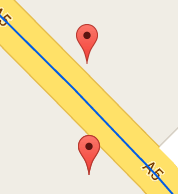
\includegraphics[scale=0.8]{collisionoffroute}
	\caption{Example of collisions excluded by the second layer of filtering when using a tolerance of 0.000001}
	\label{fig:collisionsoffroute}
\end{figure}

At this point in the development process, the collision search was functional, but there was a significant issue with performance. For long journeys, it was proving inefficient to return all collisions within the bounds of the route. This would result in tens (or even hundreds) of thousands of collisions being returned from the server. Filtering this volume of collisions using 'isLocationOnEdge' was highly inefficient, and often caused the browser to become unresponsive. It was clear that a more intelligent approach to filtering collisions in the database query was required.

\subsection{Overcoming the Performance Bottleneck}

The response returned from the Directions Service was inspected, and it was noticed that each route is split into a number of steps. As a result of this, a new approach was designed in order to produce more refined results during the initial layer of filtering. Before submitting the request to the server, bounds are calculated for each step of the route. An array containing all steps, with their bounds and coordinates, is then created. The Ajax request was updated to send this array, encoded as a JSON string, to the server. The controller decodes the JSON string and iterates through the array, calling the model to perform a search for each step. This approach returns far less invalid results, making the second layer of filtering much faster. However, it was noticed that some collisions were being incorrectly excluded as they did not pass the first layer of filtering. \autoref{fig:nonbufferedbounds} presents an example situation where this issue occurs. In the image, the black boxes represent the bounding area of two different steps. A collision that previously passed the second phase of filtering is not within the bounds of either step. In order to resolve this issue, a buffer is added to the bounds of a step before executing the database query. This means that collisions marginally outside of the bounds are still included in the results of the first layer of filtering.

\begin{figure}
	\center
	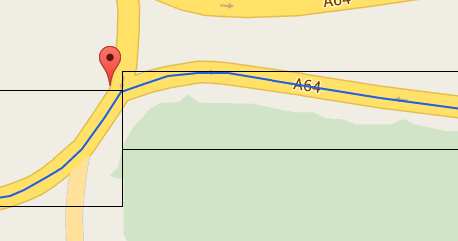
\includegraphics[scale=0.7]{nonbufferedbounds}
	\caption{Example of a valid collision excluded by the first layer of filtering}
	\label{fig:nonbufferedbounds}
\end{figure}

This change improved the performance for many routes, but the issue remained for others. This is due to the way in which different steps are defined in the response from the Directions Service. A new step is created each time a new direction is issued, which means that steps will vary considerably in terms of distance. Some routes will have a particularly long step if the route involves a long section on a motorway, for example. In an extreme case, this could lead to the database query for a step returning tens of thousands of collisions, causing the browser to become unresponsive when trying to filter these collisions. In order to prevent this, an algorithm was developed to ensure that no route step exceeds 10 kilometres in distance. A description and analysis of this algorithm is presented in \autoref{sec:restrictAlgorithm}.

This final change improved the performance considerably, ensuring that all test searches completed in under ten seconds, with the browser remaining responsive throughout. There were several challenges to overcome whilst developing this component of the system, particularly filtering database results to only include collisions near the route. This implementation has limitations in accuracy, but is far quicker and less tedious than the alternative methods available for analysing collisions on a specific route.

\subsection{Statistics Output}

The decision was made to output 5 different statistics for each search, all of which can be calculated by using data from the collisions dataset. These statistics are:

\begin{itemize}
	\item Total number of collisions.
	\item Total number of casualties.
	\item Number of collisions per kilometre.
	\item Number of casualties per kilometre.
	\item Weighted number of collisions per kilometre.
\end{itemize}

The first two are simple results to calculate, and should be of interest to most users of the application. These values are then divided by the length of the route to calculate the average number of collisions/casualties per kilometre for the route. These statistics are useful for comparing the relative safety of different routes. The anticipated use of such statistics would be for councils to compare the safety of different routes within their county, as described in Scenario A (\autoref{fig:scenarioA}). This scenario was based on information provided by West Sussex Council \citep{WestSussexCountyCouncil}, where they mention calculating and using the 'weighted casualties per km' to compare the safety of roads. Due to the time constraints of the project, increment 4 of the development cycle was not completed, so the application does not include the 'casualties' dataset. Therefore, the necessary data to compute this statistic is not available. As a viable alternative, the application calculates the 'weighted number of collisions per km'. This sums together a weighted value for each collision before dividing by the length of the route. Weighted values are assigned based on severity; 3 for fatal, 2 for serious and 1 for slight. 

Variables for the number of collisions, number of casualties, and number of weighted collisions are updated every time a collision is confirmed to be on the route. These are all divided by the length of the route after all collisions have been analysed. After all statistics have been calculated, the results are dynamically inserted into the page using jQuery.

The statistics are displayed using a HTML table, which is styled using Bootstrap \citep{Bootstrap}. As discussed in the interface design, the long statistic names are abbreviated in order to prevent the table from appearing too cluttered. The help messages were implemented using Bootstrap popovers, and are displayed when the cursor is hovered over the question mark. During testing, an issue was discovered with the display of the results table on mobile devices. The table was too wide to fit within the narrow display, requiring the user to zoom out or scroll horizontally to view everything. This problem was overcome by creating a hidden mobile-specific results table, where the axis are flipped so that there are two columns and five rows. When the screen width is below 768px, the table displayed is switched using a CSS media query.

\subsection{Heatmap}

As discussed in the design, a heatmap was used to visually represent the intensity of collisions along the route. This functionality was implemented using the Google Maps API visualisation library.

Whenever a collision is determined to be on the route, a weight is assigned to it (3 for serious, 2 for fatal and 1 for slight), and the collision is added to the heatmap data array. After all collisions have been filtered, a HeatMapLayer object is created using the heatmap data array. The HeatMapLayer is then added to the map. A coloured overlay is displayed on the map, where areas of high intensity are coloured red, and areas of low intensity are coloured green. Collisions with higher weights are rendered with greater intensity.

\subsection{Data Filters}

Filters were required for the search form so that users can specify year and severity of collisions to be included in the results. The first step of the implementation involved adding checkboxes to the search form for all available options. A validation method was added to check that at least one severity level and at least one year is selected before proceeding with a search. The validation is performed on client-side using JavaScript as soon as the form is submitted. If the validation fails, an error message explaining the problem is inserted into the page using jQuery, and the search is halted. 

If the validation passes, the selected options are inserted into two arrays, one for years and one for severity levels. These arrays are included as additional parameters when the Ajax request is sent to the server to find collisions. The model does not directly insert the arrays into the SQL query, as this would make the application vulnerable to SQL injections. To avoid this issue, a prepared statement is used as it allows the inclusion of placeholders in the SQL. Strings containing comma-separated '?' symbols, with each '?' representing an element in the original array, are dynamically created. These strings are added to the SQL query, and when the query is executed, the real values from the original arrays are inserted safely.

\section{Techniques Used}

\subsection{Importing The Data}

To make the road safety data usable by the application, it needed to be imported into a MySQL database. The STATS19 data provided by the Department for Transport contains a CSV file with all collision data for the years 2005-2013. This file was inspected to get the name and type of each field, before building a new table using MySQL Workbench. It is important to use the correct types for each field, so that data can be queried and sorted effectively. For example, storing dates of collisions using the date type allows you to query the data using year of collision. When creating the table, the 'accident index' field was assigned as the primary key, as this is the unique identifier for each collision.

A script was then created to import the data from the CSV file into the new table. An online tutorial was used to provide guidance for this task \citep{MySQLTutorial}. The date for each collision had to be transformed from 'dd/mm/yyyy' to 'yyyy-mm-dd' before inserting it into the database, in order to prevent an error from occurring.

With the data in the database, some testing was performed to find the execution times when searching for a collision using longitude and latitude values. It was noticed that this process was initially too slow, and would lead to performance issues with the application. To resolve this issue, the longitude and latitude fields in the database were indexed. After indexing these fields, the duration of queries dropped from around 2.5 seconds, to under 0.02 seconds. This is a significant performance gain, without which the final application would be almost unusable.

\subsection{Restricting The Distance of Route Steps}
\label{sec:restrictAlgorithm}

As discussed earlier in the chapter, an algorithm had to be developed in order to modify the 'steps' of a route returned from the Google Maps Directions Service. Some steps were too long, causing the database query for that step to return a large number of collisions that were far away from the route. To demonstrate this issue, the code of the application was modified to draw each step in alternate colours. \autoref{fig:longroutestep} presents a route where there is a particularly long step (drawn in red). A black rectangle has been drawn to represent the bounding area of this step. The database query returns all collisions in this bounding area, causing the browser to become unresponsive when trying to perform the second layer of filtering. 

\begin{figure}
	\center
	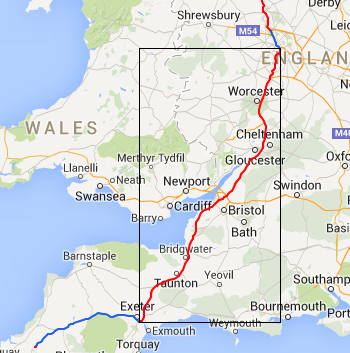
\includegraphics[scale=0.7]{longroutestep}
	\caption{Example of a long route step}
	\label{fig:longroutestep}
\end{figure}

The envisaged solution to this problem was to break a step down into several smaller steps. This leads to more database queries being executed, but more refined, and hence much fewer, results. Each step returned from the Directions Service contains a distance value and an array of coordinates, amongst other things. The application was using the array of coordinates to calculate the bounds for a step, and to draw the line on the map. In order to split the step up, it was therefore necessary to split the coordinates array and share them amongst a set of new steps. A pseudocode representation of this algorithm can be seen in Algorithm \autoref{alg:algorithm}.

\begin{algorithm}
	\caption{Splitting Route Steps}
	\label{alg:algorithm}
	\begin{algorithmic}[1]
		\Function{splitRouteSteps}{$routeSteps$}
				\State $stepCounter\gets 0$
				\ForAll{$n$ such that $0\leq n < routeSteps.length$}
					\State $distance\gets routeSteps[n].distance$
					\State $latLngs \gets routeSteps[n].lat\_lngs$
					\If{$distance> 10000$}
						\State $numberOfNewSteps\gets \lceil distance/10000 \rceil$
						\State $numberOfLatLngs\gets latLngs.length$
						\State $latLngsPerNewStep\gets \lceil numberOfLatLngs/numberOfNewSteps \rceil$
						\State $currentLatLng\gets 0$
						\ForAll{$i$ such that $0\leq i < numberOfNewSteps$}
							\State $newStepLatLngs\gets []$
							\State $j \gets 0$
							\While{$j<latLngsPerNewStep$ and $currentLatLng<numberOfLatLngs$}
								\State $newStepLatLngs[j]\gets latLngs[currentLatLng]$
								\State $currentLatLng++$
								\State $j++$
								\If{$j==latLngsPerNewStep$ and $currentLatLng<numberOfLatLngs$}
									\State $newStepLatLngs[]\gets latLngs[currentLatLng]$
									\If{$numberOfLatLngs-currentLatLng==1$}
										\State $i++$
									\EndIf
								\EndIf
							\EndWhile
							\State $newStep \gets makeStep(newStepLatLngs)$
							\State $newRouteSteps[stepCounter] \gets newStep$
							\State $stepCounter++$
						\EndFor
					\Else
							\State $newStep \gets makeStep(latLngs)$
							\State $newRouteSteps[stepCounter] \gets newStep$
							\State $stepCounter++$
					\EndIf		
				\EndFor
				\State \textbf{return} $newRouteSteps$
		\EndFunction
	\end{algorithmic}
\end{algorithm}

This algorithm takes as input an array of route steps as returned from the Directions Service. Each element of the \textit{routeSteps} array is an object comprising:
\begin{itemize}
\item A \textit{distance} field that represents the total distance for the step in metres.
\item A \textit{lat\_lngs} field that contains an array of coordinates for the step (as latitude and longitude pairs).
\end{itemize}

The algorithm returns a new array, \textit{newRouteSteps}. The new steps are created by passing the coordinates to the \textit{makeStep} function, which returns an object consisting of:
\begin{itemize}
\item A \textit{bounds} field containing the maximum and minimum latitude and longitude values for the step.
\item A \textit{lat\_lngs} field that contains an array of coordinates for the step (as latitude and longitude pairs).
\end{itemize}

The algorithm begins by initialising \textit{stepCounter}, a variable that counts how many steps have been created so far by the algorithm, to 0. The for loop in lines 3-34 iterate through all route steps. The distance of the current step and the array of coordinates are assigned to variables. A check is then made to see if the distance of the step is over 10km (line 6). If it is under 10km, the bounds of the step are calculated and it is added to the array of new steps with no further changes (lines 30-31). If the step is over this distance, it must be split into multiple smaller steps. First of all, the number of new steps is calculated by dividing the distance by 10km and rounding up to the nearest whole value (line 7). It then calculates how many pairs of coordinates should be assigned to each new step (line 9). The for loop in steps 11-28, creates each new route step. The while loop in lines 14-24 copies coordinates from the original step to the new step. The loop's conditions make it exit when the step has the maximum number of coordinates, or if there are no more coordinates to copy from the original step (line 14). After each pair of coordinates is added, a check is made to see if the new step is 'full', and there are more coordinates to copy from the original step (line 18). If this is the case, the next pair of coordinates are added to the current step. This is necessary as the steps need to be connected to each other in order to form a line for the entire route. The 'if' statement on lines 20-22 is used to ensure that a new step is not created if there is only 1 more pair of coordinates to add; this is done by incrementing $i$ so that the inner for loop terminates early. After all coordinates have been added to the new step, the bounds are calculated and it is added to the array of new steps (lines 25-26).

To analyse the time complexity of the algorithm, first note that each execution of an assignment or conditional (i.e., `if') statement requires constant, $\mathcal{O}(1)$, time. The while loop on lines 14--24 is executed at most
\[
  \mathit{latLngsPerNewStep} = \left\lceil \frac{\mathit{numberOfLatLngs}}{\mathit{numberOfNewSteps}}\right\rceil
\] 
times, and the inner for loop (lines 11--28) at most $\mathit{numberOfNewSteps}$ times, so the constant-time statements in lines 15--23 are executed
\[
 \begin{array}{ll}
  \left\lceil \frac{\mathit{numberOfLatLngs}}{\mathit{numberOfNewSteps}}\right\rceil \times \mathit{numberOfNewSteps} & \approx \mathit{numberOfLatLngs} = \\
  & = \mathit{routeSteps[n].lat\_lngs.length}
  \end{array}
\]
times. Finally, the outer for loop (lines 3--34) is executed $N=\mathit{routeSteps.length}$ times, and in the worst-case scenario $\mathit{distance}>10000$ in line 6 and the statements in lines 7--28 are carried out in every iteration of this loop. Accordingly, the overall complexity of the algorithm is $\mathcal{O}(N \cdot M)$, where 
\[
  M = \max_{0\leq n<N} \mathit{routeSteps[n].lat\_lngs.length}
\]
represents the maximum number of coordinates in a step of the processed route.

Hence the complexity of the algorithm is linear in the number of elements from $routeSteps$, and in the number of coordinates in the largest step. It is important that this algorithm is linear, so that the time taken for longer routes does not increase, for instance, exponentially.

Careful consideration had to be made when deciding upon the distance threshold used within this algorithm. A lower value leads to more refined results from the first layer of filtering, improving the time taken for the second layer of filtering. However, this also increases the number of database calls made for each route, which can have a negative effect on the performance. This creates a trade-off between the amount of computation required on client-side and sever-side. 

Response times were measured for the 20 routes specified in \autoref{tab:performanceresults1} while using different threshold values in the range 5-50. A trial and error approach was used to identify this initial range, and it was found that values either side produced longer response times. Tests were carried out for all multiples of 5 within the 5-50 range. It was concluded that 10km is the optimal threshold, as it produced results in the shortest times for most of the tested routes. A graph comparing the response times for thresholds of 5km, 10km and 15km is presented in \autoref{fig:thresholdtests}.

\begin{figure}
	\center
	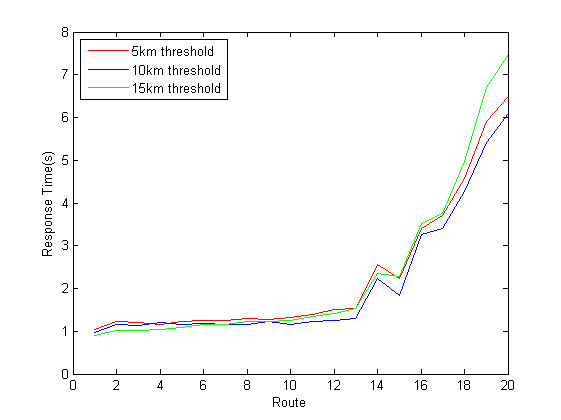
\includegraphics[scale=1]{thresholdtests}
	\caption{Graph showing response times for different distance thresholds}
	\label{fig:thresholdtests}
\end{figure}

 \autoref{fig:shortersteps} shows the results of running this algorithm on the long route step from \autoref{fig:longroutestep}. Black rectangles have been drawn to represent the bounding areas of each of the new steps. This clearly demonstrates that far less invalid collisions will be returned as a much smaller area is being analysed.

\begin{figure}
	\center
	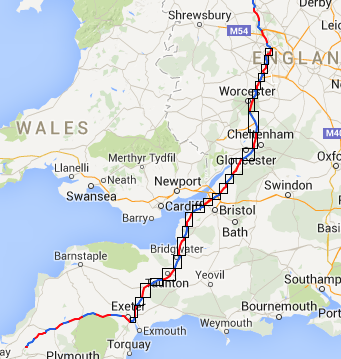
\includegraphics[scale=0.7]{shortersteps}
	\caption{Example of route steps after using the splitRouteSteps function}
	\label{fig:shortersteps}
\end{figure}

\section{Summary}
This chapter discussed the challenges faced during the implementation of Route Risks, and the solutions used to overcome them. There is a focus on the collision searching functionality as this is unique to this application and provided the most interesting challenges during development. The next chapter focuses on testing and evaluating the system.

\chapter{Testing and Evaluation}

\section{Testing and Evaluation Methodology}

The testing and evaluation of the road safety advisory system was conducted in four primary stages:

\begin{enumerate}
	\item Functional testing - A series of test cases have been designed to test that the system produced meets its functional requirements. These tests do not require knowledge of the code, and are focused on ensuring that everything is functional from the perspective of a user (black-box testing). After each increment of the system was developed, the relevant tests for the new functionality were run, along with tests for existing functionality. This regression testing ensures that code changes do not break previously functional parts of the application.
	\item Accuracy testing - One of the main challenges of testing the application involves checking that the results produced are accurate. As there is not an existing application that performs collision searching by route, there is no basis for comparison. Hence the decision was made to use Crash Map \citep{crashmap} in order to manually zoom/pan along a route and count the number of collisions. The results, and time taken to calculate them, are compared with the results obtained using Route Risks.
	\item Performance testing -  Performance analysis was carried out to determine how fast the system is, and to determine what impacts the speed. The aim of this analysis is to ensure that the system is fully scalable. 
	\item Usability testing - User evaluations were carried out to test the usability of the application. Participants were asked to perform a set of tasks using the application and raise any usability issues.
\end{enumerate}

\section{Testing and Evaluation Environment}

Prior to testing, the application was deployed onto an EC2 instance provided by Amazon Web Services \citep{AmazonWebServices}. All testing was performed by accessing the application via this server. The Database was hosted on an RDS instance, also provided by Amazon Web Services. The specifications of these servers are presented in \autoref{tab:serverspecs} and \autoref{tab:dbserverspecs}.

\begin{table}
	\center
	\caption{Web server specifications}
	\label{tab:serverspecs}
	\begin{tabular}{| p{4cm} | p{9cm} |}
	\hline
	\textbf{Instance Type} & t2.micro (Variable ECUs, 1 vCPUs, 2.5 GHz, Intel Xeon Family, 1 GiB memory, EBS only) \\ \hline
	\textbf{Operating System} & Ubuntu Server 14.04 LTS \\ \hline
	\textbf{Deployed Components} & Apache, PHP, Git, Route Risks. \\ \hline
	\end{tabular}
\end{table}

\begin{table}
	\center
	\caption{Database server specifications}
	\label{tab:dbserverspecs}
	\begin{tabular}{| p{4cm} | p{9cm} |}
	\hline
	\textbf{Instance Type} & db.t2.micro - 1 vCPU, 1 GiB RAM \\ \hline
	\textbf{DB Engine} & MySQL  5.6.22 \\ \hline
	\end{tabular}
\end{table}

This is the intended final deployment of Route Risks, and its end users can currently access the application at \url{RouteRisks.co.uk} (\autoref{fig:routerisks}).

\begin{figure}
	\center
	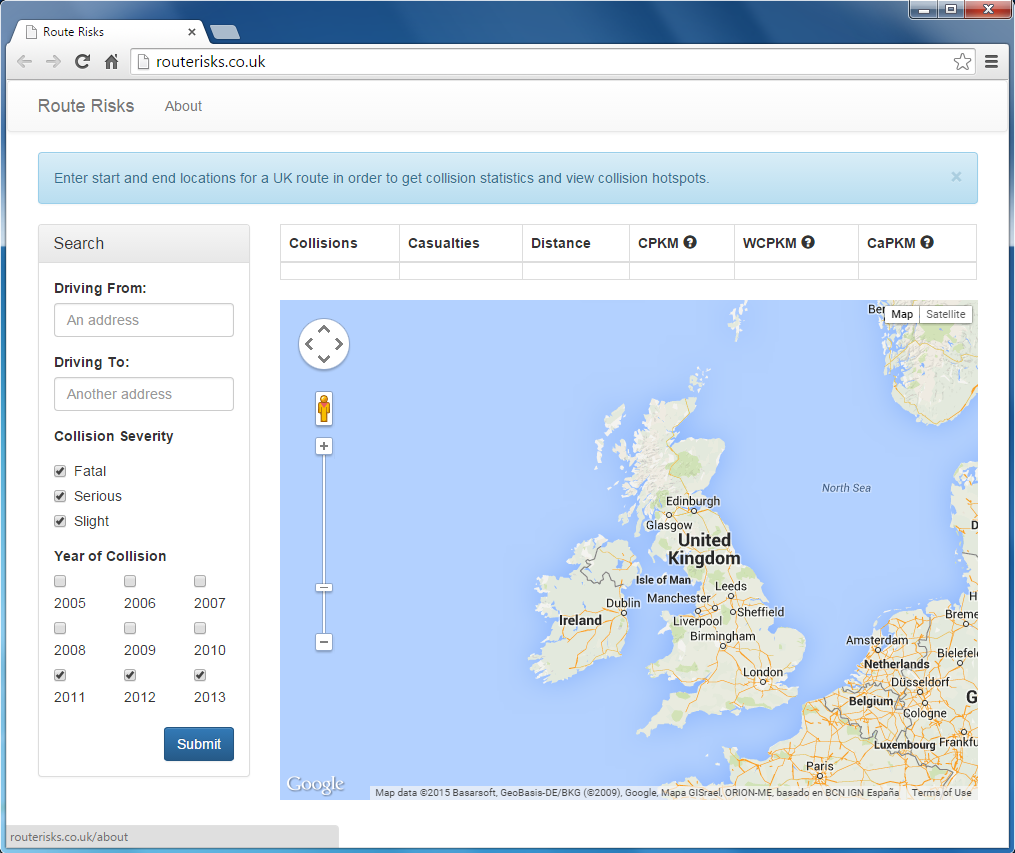
\includegraphics[scale=0.55]{routerisks}
	\caption{Route Risks application accessed at \url{RouteRisks.co.uk}}
	\label{fig:routerisks}
\end{figure}

\section{Functional Testing}

Test cases were written to test each functional requirement specified in \autoref{tab:FunctionalReqs}. Each table presented later in this section specifies a test case, which consists of a description, test steps, expected outcome, and passing criteria.

Test cases 1 to 6 were designed to test the functionality of the application using only its user interface. Therefore, these tests were carried out in the latest versions of Google Chrome, Mozilla Firefox and Internet Explorer. They were also carried out on mobile Safari using an iPhone 5 in both vertical and horizontal mode. This approach is required in order to confirm that the application is compatible with different browsers and devices, which is necessary due to NFR1 and NFR8 (\autoref{tab:NonFunctionalReqs}).

TC-007 requires the use of developer tools in the browser in order to inspect the response from the web server, so was only performed in Google Chrome. This test is necessary to ensure that the data filters are working correctly. The data filters are also (indirectly) tested in \autoref{sec:searchAnalysis} as different filters are used when analysing the accuracy of the collision search.

The remainder of this section describes each test case. All of the test cases passed when carried out on the final build of the application.

\begin{tabular}{| p{2.5cm} | p{11cm} |}
	\hline
	\textit{Test Case ID} & TC-001 \\ \hline
	\textit{Requirement(s) Covered} & FR1, FR2 \\ \hline
	\textit{Description} & Check that it is possible to search UK road safety data using a route between two locations.  \\ \hline
	\textit{Test Steps}& - Enter a start and end location.
	\newline - Submit the search.
	\newline - Verify that results returned are for the route entered.
 \\ \hline
	\textit{Expected Outcome} & The application uses the route to search for collisions, and presents the results to the user.  \\ \hline
	\textit{Pass Criteria} & The user is presented with results relevant to the entered route.  \\ \hline
\end{tabular}

\begin{tabular}{| p{2.5cm} | p{11cm} |}
	\hline
	\textit{Test Case ID} & TC-002 \\ \hline
	\textit{Requirement(s) Covered} & FR1, FR2, FR6 \\ \hline
	\textit{Description} & Check that statistics are calculated when searching UK road safety data using a route between two locations.  \\ \hline
	\textit{Test Steps}& - Enter start/end locations and submit a search.
	\newline - Verify that statistics including number of collisions, collisions per kilometre (CPKM), weighted CPKM, casualties and casualties per kilometre (CaPKM) are all calculated.
	\newline - Verify that $\frac{Collisions}{Distance} = CPKM $ and $\frac{Casualties}{Distance} = CaPKM$
 \\ \hline
	\textit{Expected Outcome} & The application uses the route to search for collisions and calculate the relevant statistics before presenting the results to the user.  \\ \hline
	\textit{Pass Criteria} & The user can see each of the relevant statistics in a table. The distance has been used to calculate CPKM and CaPKM. \\ \hline
\end{tabular}


\begin{tabular}{| p{2.5cm} | p{11cm} |}
	\hline
	\textit{Test Case ID} & TC-003 \\ \hline
	\textit{Requirement(s) Covered} & FR1, FR2, FR4 \\ \hline
	\textit{Description} & Check that collision density is represented on an interactive map when searching for collisions between two locations.  \\ \hline
	\textit{Test Steps}& - Enter start/end locations and submit a search.
	\newline - Verify that the route is displayed on the map, with a clear indication of where most collisions occur.
	\newline - Verify that it is possible to interact with the map by zooming and panning. 
 \\ \hline
	\textit{Expected Outcome} & The application uses the route to search for collisions, displays the route on the map, and produces a heatmap to visualise the intensity of collisions along the route.  \\ \hline
	\textit{Pass Criteria} & The user can interact with a map, which displays the route and a heatmap. The heatmap highlights sections of the route with the most collisions using red, whilst sections with less collisions are green.  \\ \hline
\end{tabular}

\begin{tabular}{| p{2.5cm} | p{11cm} |}
	\hline
	\textit{Test Case ID} & TC-004 \\ \hline
	\textit{Requirement(s) Covered} & FR1, FR2, FR3, FR5 \\ \hline
	\textit{Description} & Check that it is possible to immediately submit a new search after a previous search has completed. \\ \hline
	\textit{Test Steps}& - Enter start/end locations and submit a search.
	\newline - Verify that results returned are for the route entered.
	\newline - Enter different start/end locations and submit a search.
	\newline - Verify that previous results are cleared and new results are displayed.
 \\ \hline
	\textit{Expected Outcome} & The application clears the results of a search when a new search is submitted.  \\ \hline
	\textit{Pass Criteria} & The user sees the results change after submitting a different search.  \\ \hline
\end{tabular}

\begin{tabular}{| p{2.5cm} | p{11cm} |}
	\hline
	\textit{Test Case ID} & TC-005 \\ \hline
	\textit{Requirement(s) Covered} & FR1, FR2, FR7 \\ \hline
	\textit{Description} & Check that it is possible to filter collisions included in results by year. \\ \hline
	\textit{Test Steps}& - Enter start/end locations, choose a selection of years, and submit a search.
	\newline - Verify that results returned are for the route entered.
	\newline - Change the selection of years
	\newline - Verify that the results produced correctly reflect the number of years selected.
	\newline - Repeat the previous 2 steps five times.
 \\ \hline
	\textit{Expected Outcome} & The application uses the years selected by the user to filter collision results.  \\ \hline
	\textit{Pass Criteria} & The results produced by the application reflect the selection of years. The number of collisions found for a selection of years is equal to the number of collisions found for each year individually.  \\ \hline
\end{tabular}

\begin{tabular}{| p{2.5cm} | p{11cm} |}
	\hline
	\textit{Test Case ID} & TC-006 \\ \hline
	\textit{Requirement(s) Covered} & FR1, FR2, FR6, FR8 \\ \hline
	\textit{Description} & Check that it is possible to filter collisions included in results by severity, and that weighted CPKM is calculated correctly. \\ \hline
	\textit{Test Steps}& - Enter start/end locations, select slight severity, and submit a search.
	\newline - Verify that results returned are for the route entered and that the Weighted CPKM is equal to the CPKM.
	\newline - Change the severity selection to serious.
	\newline - Verify that results returned are for the route entered and that the Weighted CPKM is double the CPKM.
	\newline - Change the severity selection to fatal.
	\newline - Verify that results returned are for the route entered and that the Weighted CPKM is triple the CPKM.
	\newline - Change the severity selection to all severities.
	\newline - Verify that results returned are for the route entered and that the Weighted CPKM is equal to the previous 3 added together.
 \\ \hline
	\textit{Expected Outcome} & The application uses the severity levels selected by the user to filter collision results.  \\ \hline
	\textit{Pass Criteria} & The results produced by the application reflect the selection of severities. The weighted CPKM is calculated according to the users selection each time. \\ \hline
\end{tabular}

\begin{tabular}{| p{2.5cm} | p{11cm} |}
	\hline
	\textit{Test Case ID} & TC-007 \\ \hline
	\textit{Requirement(s) Covered} & FR1, FR2, FR7, FR8 \\ \hline
	\textit{Description} & Check the response from the server to ensure that date and severity are filtered correctly. \\ \hline
	\textit{Test Steps}& - Access the Google Chrome Developer tools to view network requests. 
	\newline - Enter start/end locations, choose a selection of severity levels and years, and submit the search.
	\newline - View the 'getcollisions' request and access the response.
	\newline - Verify that there is an array of collision objects, with each object containing an accident index, longitude, latitude, severity and number of casualties.
	\newline - Verify that the first 4 characters of all accident indexes correspond to a year that was selected in the search parameters.
	\newline - Verify that all accident severity values correspond to the severity levels selected in the search parameters (where 1 is fatal, 2 is serious and 3 is slight).
	\newline - Repeat this test 5 times using different search parameters.
 \\ \hline
	\textit{Expected Outcome} & The application uses the severity levels and years selected by the user to filter collision results.  \\ \hline
	\textit{Pass Criteria} & The response from the server only contains results for the selected years and severity levels. \\ \hline
\end{tabular}

\section{Accuracy}
\label{sec:searchAnalysis}

In order to evaluate how successful the method used for collision searching is, it is important to analyse the accuracy of the results. The implementation is not expected to be 100\% accurate due to the following issues:

\begin{itemize}
	\item The accuracy of the latitude/longitude values recorded for each collision cannot be guaranteed. If the values recorded are far enough away from the road, they will be excluded from the results.
	\item The application will include all collisions within a certain distance of the route. This can lead to collisions on different roads being included.
\end{itemize}

This section of the report includes a description of the method used to test the accuracy, and a discussion of the results.

\subsection{Method}

The accuracy of the application was tested by comparing the results of Route Risks with those manually obtained using Crash Map \citep{crashmap}. The following process was followed for each test route:

\begin{enumerate}
	\item Access Crash Map and search for the start of the route. Adjust the data filters accordingly.
	\item Follow the route by panning and zooming on the map where necessary. Count the number of collisions on the route.
	\item Record the total number of collisions found, and the time taken to carry out the search (to the nearest second).
	\item Access Route Risks and perform a search using the specified details.
	\item Record the total number of collisions found, and the time taken to carry out the search (to the nearest second).
\end{enumerate}

15 test routes were prepared for analysing the accuracy of the application. The locations of the routes were picked randomly from anywhere in the UK. These tests focused on short distance routes (all under 20km, with the majority under 10km) because manually counting CrashMap collisions is a tedious, time-consuming process that was not feasible for long routes within the timeframe of the project. The test routes are specified in \autoref{tab:accuracyroutes}.

\begin{table}
	\center
	\caption{Routes used for testing collision search accuracy}
	\label{tab:accuracyroutes}
	\begin{tabular}{| l | l | l | l |}
	\hline
	\textbf{Route ID} & \textbf{Start Location} & \textbf{End Location} & \textbf{Distance (km)}  \\ \hline
	1 & Mulgrave St, Hull & Shaw St, Hull & 0.9  \\ \hline 	
	2 & Edwin Road, Leeds & Hyde Terrace, Leeds & 1.2  \\ \hline 
	3 & Merthyr Tydfil & Pen-y-Darren & 1.3  \\ \hline 
	4 & YO31 0SH & YO10 5NL & 1.9 \\ \hline
	5 & M5 3AW & M5 4LT & 2.2  \\ \hline 
	6 & N1 0QH & N1 5PH & 2.3 \\ \hline
	7 & Bowburn, Durham & Coxhoe, Durham & 2.5  \\ \hline 
	8 & LL60 6HR & LL60 6NN & 3.3  \\ \hline 
	9 & Welbeck Rd, Newcastle & Fairburne Avenue, Newcastle & 3.8  \\ \hline 
	10 & Holt Heath & Little Witley & 4.1 \\ \hline
	11 & PH5 2AB & PH7 4HL & 4.1 \\ \hline
	12 & PL3 6RW & PL3 5BD & 4.8  \\ \hline 
	13 & ML3 6AD & ML2 0EQ & 7.7  \\ \hline 
	14 & YO19 4TA & YO19 5UP & 9  \\ \hline 
	15 & Llanfyllin & Welshpool & 18.5  \\ \hline 
	\end{tabular}
\end{table}

\subsection{Results}

The results of the tests are presented in \autoref{tab:accuracyresults}. For four of the 15 tested routes, the number of collisions found using both applications was the same. For three of the routes, the number of collisions found differed by one, and for five it differed by two. The graph shown in \autoref{fig:graphaccuracy} demonstrates how the number of collisions found for a route differs between the two applications. There is a strong positive correlation between the two sets of results, and the line of best fit is close to $y=x$. This shows that, on average, the application returns the correct number of collisions. These results give confidence that the application is operating accurately, although more testing, including for longer routes, is required to improve the level of confidence in these preliminary results.

\begin{table}
	\center
	\caption{Comparison of results from Crash Map and Route Risks}
	\label{tab:accuracyresults}
	\begin{tabular}{| p{1cm} | p{2cm} | p{2.5cm} | p{1.7cm} | p{1.7cm} | p{1.7cm} | p{1.7cm} |}
	\hline
	\multicolumn{3}{|c|}{} & \multicolumn{2}{c|}{\textbf{Crash Map}} & \multicolumn{2}{c|}{\textbf{Route Risks}}  \\ \hline
	Route & Years & Severity Levels & Collisions & Time(s) & Collisions & Time(s) \\ \hline
	1 & All & All & 29 & 73 & 30 & 1 \\ \hline
	2 & All & All &16 & 78 & 19 & 1 \\ \hline
	3 & 2012 & Slight & 4 & 13 & 3 & 1 \\ \hline
	4 & 2009-13 & All & 9 & 105 & 11 & 1 \\ \hline
	5 & 2011-13 & All & 11 & 72 & 9 & 1 \\ \hline
	6 & All & Serious & 7 & 163 & 11 & 1 \\ \hline
	7 & 2012-13 & All & 5 & 41 & 5 & 1 \\ \hline
	8 & 2005, 2007, 2009 & All & 3 & 25 & 1 & 1 \\ \hline
	9 & 2008-10 & Slight, Serious & 22 & 148 & 14 & 1 \\ \hline
	10 & All & Slight & 6 & 92 & 8 & 1 \\ \hline
	11 & All & All & 2 & 85 & 2 & 1 \\ \hline
	12 & All & Serious, Fatal & 6 & 35 & 6 & 1 \\ \hline
	13 & 2011-13 & Serious, Fatal & 2 & 113 & 2 & 1 \\ \hline
	14 & All & Fatal & 2 & 74 & 0 & 1 \\ \hline
	15 & 2010-13 & Serious, Fatal & 3 & 131 & 2 & 1 \\ \hline
	\end{tabular}
\end{table}

\begin{figure}
	\center
	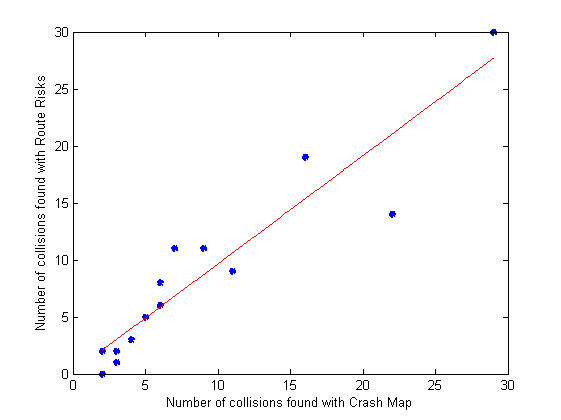
\includegraphics[scale=1]{accuracycomparison}
	\caption{Graph comparing the results from \autoref{tab:accuracyresults}}
	\label{fig:graphaccuracy}
\end{figure}

\subsection{Discussion}

The use of Crash Map to analyse the accuracy of the application has a number of issues. Firstly, the application is not designed to analyse routes in this manner, so there is not an automated process. Therefore, it is open to human error when counting up the number of collisions. Three of the tests carried out had to be restarted after forgetting how many collisions had been counted mid-way through. It is also down to the user to make a decision as to whether a collision is on the route or not. In many cases this will be obvious, but when a collision is on a junction between the route and an adjoining road, for example, some users may choose to include it in the results, whilst some may exclude it. Because of these factors, the results obtained when using Crash Map cannot be accepted as conclusively correct. However, as there is no better approach available, these figures are considered as correct for the basis of this experiment.

Another issue with using Crash Map for these tests is the time taken. Manually navigating the route, and waiting for collisions to load each time the map is panned/zoomed is a long and tedious process. The results in \autoref{tab:accuracyresults} show that the time taken for each search ranged from 13 seconds to 2 minutes and 43 seconds. This issue would be accentuated further for longer routes. In comparison, Route Risks completed all searches in 1 second. 

It is important to understand why the system sometimes returns too many or too few collisions. To do this, some of the routes tested were examined further. \autoref{fig:excludedcollisionsroute8} shows the 2 collisions that were included in the results for route 8 when testing with Crash Map, but excluded by Route Risks. Both collisions are plotted a considerable distance away from the road. A human viewing these points will still associate them with the route, because there is not another road nearby. However, the automated filtering performed by Route Risks will determine that they are too far away from the route to be relevant. This could be resolved by increasing the tolerance value used when filtering collisions, but this could have an adverse affect when analysing other routes.

\begin{figure}
	\center
	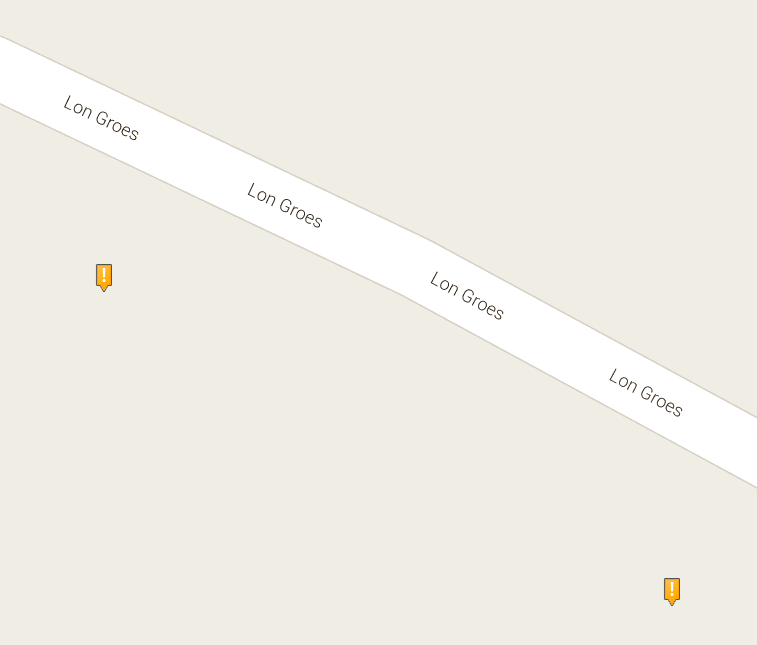
\includegraphics[scale=0.5]{excludedcollisions}
	\caption{Collisions excluded when testing route 8 in Route Risks (screen shot from Crash Map \citep{crashmap})}
	\label{fig:excludedcollisionsroute8}
\end{figure}

\autoref{fig:includedcollisionroute6} shows a collision that is included in the results for route 6 by Route Risks, but excluded by the user when using Crash Map. To a user viewing the map it is clearly not on the route, but to the system it is considered close enough to the route to be relevant. An increase in the tolerance value to resolve the issue for route 8 would ultimately lead to more issues like this. Hence the tolerance value used is a trade-off, as it can lead to too many or too few collisions being included in the results for any given route. These tests suggest that the tolerance value used is suitable as Route Risks' results are, on average, equivalent to the results found using Crash Map. 

\begin{figure}
	\center
	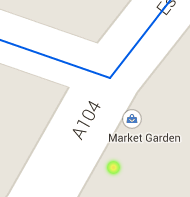
\includegraphics[scale=1]{incorrectlyincluded}
	\caption{Collision wrongly included when testing route 6 in Route Risks}
	\label{fig:includedcollisionroute6}
\end{figure}

Whilst carrying out these tests, it was noticed that a large proportion of collisions are plotted far away from roads on both Crash Map and Route Risks. It is possible that the collision data provided is not accurate enough, which increases the difficulty of automatically filtering collisions by route. Open data accuracy is a general concern, as discussed in the literature review (\autoref{sec:openDateBenefits&Challenges}). Another possible cause for these issues is the Google Maps API not correctly projecting the points onto the map. Further work is required in order to investigate these theories.

\section{Performance}

It is important to test the performance of the application for a number of routes in order to prove its scalability. It is reasonable to expect that longer routes will take longer to search as there is more data to process. However, it is important that the application is still able to respond in under 10 seconds for all routes, as specified by NFR4. 

\subsection{Method}

Twenty test routes were prepared for analysing the performance of the application. The locations of the routes were picked randomly from anywhere within the UK. The distances of the routes were highly influential during this process, as it was important to have a good variety. The routes vary in distance from 1.9km to 949km, with the majority under 50km as longer journeys are less likely to be important to users (e.g. councils looking to analyse routes within their county will not need to look at routes that are several hundreds of kilometres). \autoref{fig:routerisksshort} and \autoref{fig:routeriskslong} show the results produced by Route Risks for the shortest (1.9km) and the longest (949km) routes used for the performance evaluation, respectively.


\begin{figure}
	\center
	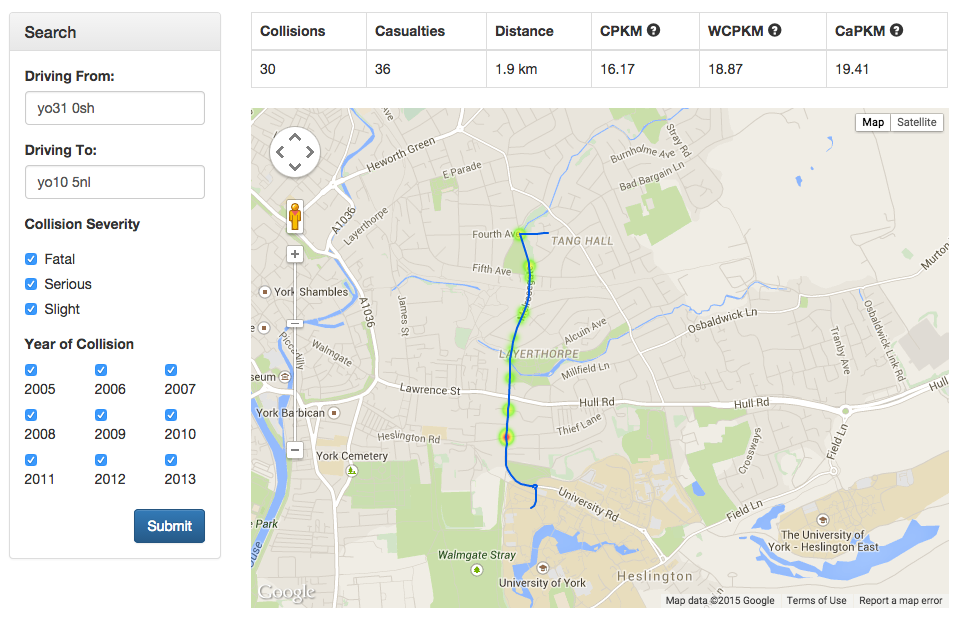
\includegraphics[scale=0.45]{routerisksshortdist}
	\caption{Route Risks results for a short journey}
	\label{fig:routerisksshort}
\end{figure}

\begin{figure}
	\center
	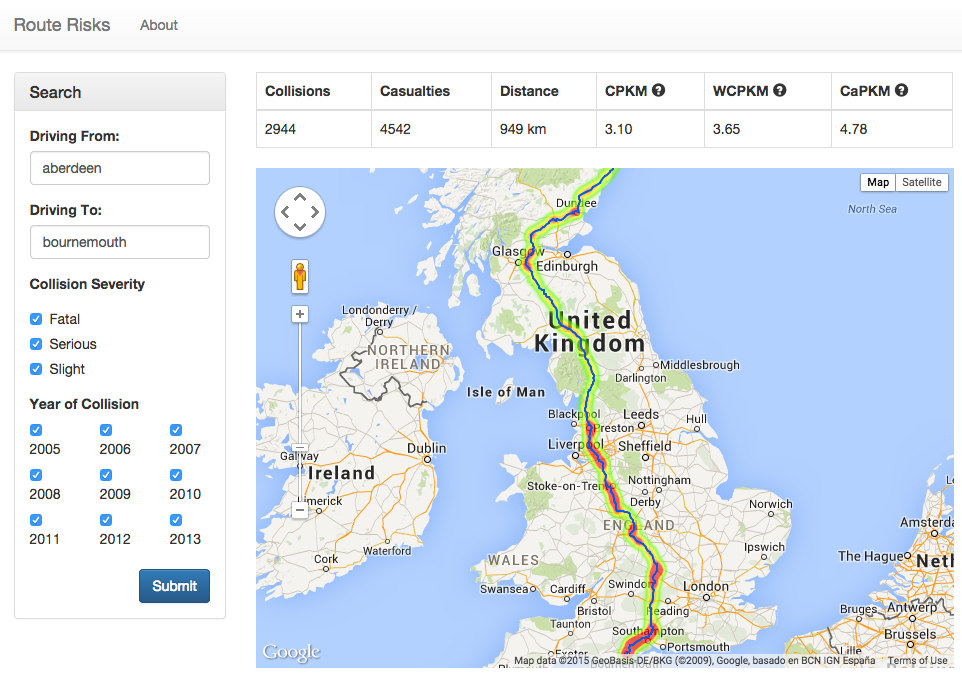
\includegraphics[scale=0.45]{routeriskslongdist}
	\caption{Route Risks results for a long journey}
	\label{fig:routeriskslong}
\end{figure}

The first tests focused purely on comparing response times for different distances. Hence, all severity levels and years were included in the searches to ensure a controlled experiment. Including data for all years and severity levels also ensures that the maximum amount of data is returned for each route, which should also lead to the worst-case response times. 

The second tests focused on comparing response times for a different selection of years. Hence, all severity levels were included and the same route was used each time to ensure a controlled experiment. This test was performed for three different routes from the list of twenty. The routes were selected based on their distances in order to evaluate how the number of years affects response times for routes of different lengths.

Response time was measured manually using a stop watch. The stop watch was started as soon as the search was submitted, and stopped as soon as the results were presented on the screen. Measuring time manually like this can be inaccurate as it relies on human reaction speed. To improve the reliability of the results, each test was performed five times and the average response time was taken.

\subsection{Results}

The results of the first set of tests are presented in \autoref{tab:performanceresults1}. As expected, there is a strong positive correlation between response times of the system and the distance of the route being analysed. Crucially, the longest route analysed completed in 6.1 seconds, which is considerably below the target of 10 seconds. \autoref{fig:graphrespdist} presents a graph to better demonstrate the relationship between distance and response time. Each of the results has been plotted and a line of best fit has been drawn using the data. This line can be used to estimate the response time for a route, given its distance. The equation of the line is as follows:
$$ Response Time = 0.0057\times Distance + 1.14$$

where the response time is expressed in seconds, and the distance in kilometres.

It is possible to use this empirically-derived equation to estimate what distance a route must be in order to exceed a response time of 10 seconds. This analysis suggests that searches for routes under 1500km in length will complete in under 10 seconds, assuming that the user's connection is not the bottleneck. The route from Land's End in South-West England to John O'Groats in North-East Scotland is widely considered to be the longest point-to-point route on the island of Great Britain, at a distance of 1348km. This suggests that the application will always respond in under 10 seconds, as no route in the UK is longer than 1500km. The route mentioned here was tested and the system responded in 6.3 seconds. 

\begin{table}
	\center
	\caption{Comparison of response times for different routes}
	\label{tab:performanceresults1}
	\begin{tabular}{| l | l | l | l |}
	\hline
	\textbf{Start Location} & \textbf{End Location} & \textbf{Distance (km)} & \textbf{Response Time (s)} \\ \hline
	YO31 0SH & YO10 5NL & 1.9 & 0.98 \\ \hline
	N1 0QH & N1 5PH & 2.3 & 1.16 \\ \hline
	Holt Heath & Little Witley & 4.1 & 1.13 \\ \hline
	PH5 2AB & PH7 4HL & 4.1 & 1.2 \\ \hline
	ML3 6AD & ML2 0EQ & 7.7 & 1.16 \\ \hline 
	Knutsford & Chelford & 8.2 & 1.18 \\ \hline
	Baschurch & Shrewsbury & 13.8 & 1.16 \\ \hline
	CA8 1GH & CA1 2PD & 17.5 & 1.15 \\ \hline
	Guildford & Farnborough & 21.2 & 1.23 \\ \hline
	Ashford & Folkestone & 24.8 & 1.15 \\ \hline
	Chesterfield & Buxton & 39.5 & 1.23 \\ \hline
	Bala, Gwynedd & Barmouth & 44.2 & 1.26 \\ \hline
	Liverpool & Manchester & 54.9 & 1.3 \\ \hline
	Nottingham & Leeds & 115 & 2.23 \\ \hline
	Plymouth & Bristol & 195 & 1.84 \\ \hline
	London & Sheffield & 260 & 3.26 \\ \hline
	Portsmouth & Lincoln & 350 & 3.4 \\ \hline
	Swansea & Norwich & 497 & 4.26 \\ \hline
	Exeter & Glasgow & 719 & 5.41 \\ \hline
	Aberdeen & Bournemouth & 949 & 6.1 \\ \hline
	\end{tabular}
\end{table}

\begin{figure}
	\center
	\includegraphics[scale=1]{performance-distance-responsetime}
	\caption{Graph demonstrating the relationship between response time and route distance}
	\label{fig:graphrespdist}
\end{figure}

The results for the second part of the performance analysis are presented in \autoref{tab:performanceresults2}. It is clear that there is a positive correlation between the number of years selected and the response time. This correlation becomes stronger for longer routes. The graph in \autoref{fig:graphrespyears} includes a line for each route, demonstrating how the response time changes as the number of years selected is changed. The shortest route shows little overall change in response time, whilst the longest route has a difference of almost 3 seconds from when there is just 1 year selected to when all 9 years are selected. This is because the difference in collisions found for the shortest route is only 238, whilst the difference for the longest route is 2406. This proves that distance is not the only influence on performance, and that the number of collisions found for the route also has a significant impact.

\begin{table}
	\center
	\caption{Comparison of response times when the 'Year of Collision' filter is changed}
	\label{tab:performanceresults2}
	\begin{tabular}{| l | l | l | l | l |}
	\hline
	\textbf{Start Location} & \textbf{End Location} & \textbf{Distance (km)} & \textbf{Years} & \textbf{Response Time (s)} \\ \hline
	Guildford & Farnborough &  21.2 & 2013 & 1.03 \\ \hline
	 &  &  & 2011-2013 & 1.1 \\ \hline
	 &  &  & 2008-2013 & 1.2 \\ \hline
	 &  &  & 2005-2013 & 1.23 \\ \hline
	 London & Sheffield &  260 & 2013 & 1.76 \\ \hline
	 &  &  & 2011-2013 & 2.15 \\ \hline
	 &  &  & 2008-2013 & 2.46 \\ \hline
	 &  &  & 2005-2013 & 3.26 \\ \hline
	 Exeter & Glasgow &  719 & 2013 & 2.65 \\ \hline
	 &  &  & 2011-2013 & 3.31 \\ \hline
	 &  &  & 2008-2013 & 4.06 \\ \hline
	 &  &  & 2005-2013 & 5.41 \\ \hline
	\end{tabular}
\end{table}

\begin{figure}
	\center
	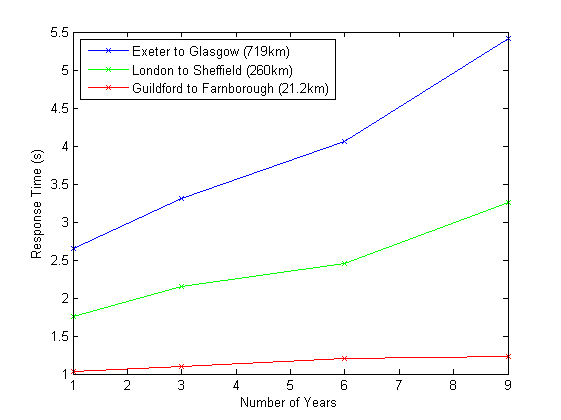
\includegraphics[scale=1]{performance-years}
	\caption{Graph demonstrating the relationship between response time and number of years specified}
	\label{fig:graphrespyears}
\end{figure}

It is also worth consideration that other factors can impact the performance of the application, which may cause an increase in response times. A poor connection on the user's end may lead to slow download times which could significantly affect the performance for them. Furthermore, if there are a large number of users on the site concurrently, response times from the server may increase. However, this problem can be addressed easily since Route Risks is deployed on public cloud infrastructure and can therefore be scaled up to run on multiple virtual machines, albeit at additional cost.


\section{User Evaluation}

When an application is deemed to be sufficient by the developer, it is necessary to test it with real users \citep{Cooper2007}. A small summative evaluation was carried out on the final version of Route Risks in order to evaluate the usability. 

\subsection{Method}

The user evaluations were carried out by asking users who had no prior knowledge of the application to complete a set of tasks. Users were only given a brief introduction to the site, which purposely held back information so that they would read help messages or the 'about' page if necessary. This was done in order to test NFR3 and NFR4, which state that users should be able to use the application without external assistance, and that results should be presented in a user-friendly manner. Users were asked to discuss their thought process while carrying out the tasks by using a concurrent verbal protocol. Any usability issues found were discussed and given a severity rating using the scale defined by Nielsen \citep{Nielsen1995}; 1 for cosmetic problems, 2 for minor usability problems, 3 for major usability problems and 4 for usability catastrophes.

All participants were briefed on the process used and informed that their responses would be completely anonymous. They were then asked to sign a consent form in order to confirm their understanding. 

All users used the same testing environment; a Windows 7 PC with a 23" monitor, running a maximised Google Chrome window. The application was accessed via \url{routerisks.co.uk}.

The users were asked to complete the following tasks:

\begin{enumerate}
	\item Search for all collisions between Thirsk and Scarborough between 2011 and 2013 and point out where the collision hotspots are for the route.
	\item In a separate browser tab, search for all collisions between Bridlington and Scarborough between 2011 and 2013.
	\item Compare the results of the two searches and discuss which route is the most dangerous to drivers.
\end{enumerate}

These routes were chosen in order to see how users would use the statistics when comparing the danger of routes. The first route is far longer than the second, and has double the number of collisions/casualties. However, the second route has higher 'per kilometre' values. It was therefore interesting to evaluate which statistics users preferred to use as a basis for the comparison.

\subsection{Results}

A total of six participants took part in the user evaluation. The usability issues raised are presented in \autoref{tab:userevalprobs}. A total of 7 unique issues were raised, and all of these were assigned severity ratings of 1 or 2. One user did not raise any issues. The most common problem was that users wanted to see the distance of the routes when carrying out the comparison. As this issue was raised by 50\% of the participants, it was deemed a high priority, so a fix was immediately implemented. This was done by adding a 'distance' column to the results table. \autoref{fig:resultstablebefore} shows the results table before this fix, and \autoref{fig:resultstableafter} shows the changes made following the user feedback. In addition to adding a 'distance' field, the fields were rearranged into a more logical order.

\begin{figure}
	\center
	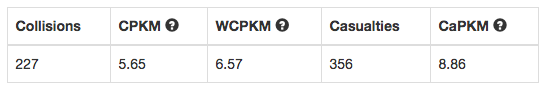
\includegraphics[scale=0.75]{resultstablebefore}
	\caption{Route Risks results table before user evaluation}
	\label{fig:resultstablebefore}
\end{figure}

\begin{figure}
	\center
	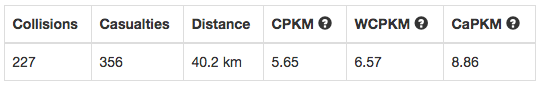
\includegraphics[scale=0.75]{resultstableafter}
	\caption{Route Risks results table following usability improvement}
	\label{fig:resultstableafter}
\end{figure}

Other issues were considered less important as they were only raised by a single user and were not assigned a high severity rating. However, these issues are still worth consideration for future work.

\begin{table}
\caption{User Evaluation Problems}
\begin{tabular}{| p{1.5cm} | p{1.5cm} | p{9cm} | p{1.5cm} |}
	\hline
	\textbf{Problem No.} & \textbf{User No.} & \textbf{Problem Description} & \textbf{Severity Rating} \\ \hline
	1 & 1 & The user expected the locations field to provide a list of suggestions as they typed, as this is a common feature in other applications (such as Google Maps)  & 2 \\ \hline
	2 & 1 & The user was unsure what the definition of a 'serious' collision was, and would have liked a description of the different severity levels. & 1 \\ \hline
	3 & 1 & The user wanted to see the distance of the routes when carrying out the comparison. & 2 \\ \hline
	4 & 2 & The user felt it was unclear what the different colours of the heatmap represented. They believed that a scale should be presented giving details of how many collisions each colour represents. & 2 \\ \hline
	5 & 3 & The user did not like how the heatmap updates on zooming. They found it confusing that sections of the route in red were no longer red after zooming in.  & 1 \\ \hline
	6 & 4 & The user wanted to see the distance of the routes when carrying out the comparison. & 2 \\ \hline
	7 & 5 & The user wanted to view the road name when hovering over a collision hotspot. & 2 \\ \hline
	8 & 5 & The user wanted to see the distance of the routes when carrying out the comparison. & 2 \\ \hline
	9 & 5 & The user felt as though it wasn't obvious which statistics were the most important when comparing the danger of 2 routes. & 1 \\ \hline
\end{tabular}
\label{tab:userevalprobs}
\end{table}

The following additional observations were made whilst the users carried out the tasks:

\begin{itemize}
	\item All users concluded that the second route was the most dangerous as it has the highest 'per kilometre' statistics, and a higher proportion of the route is displayed in red.
	\item Four of the users became completely immersed while using the interactive map, and took a long time to notice the presence of the statistics. 
	\item After noticing the statistics, users had no issues with understanding what each statistic meant. They immediately recognised that the acronyms would be explained by hovering over the '?' symbol.
	\item Only one of the users read the help message at the top of the page. This user was also the only one to immediately check the statistics after submitting a search.
	\item All users felt comfortable using the interface without any assistance.
\end{itemize}

Whilst all users were comfortable using the application, it must be taken into consideration that all 6 participants were final-year computer science students. The participants all have strong technical skills and are familiar with using various web applications. It is almost certain that many future users of the application will not be as skilled, and hence may encounter more issues. It would be a valuable exercise to carry out this user evaluation with more participants, covering a larger demographic.

The technical experience of the users also explains why so many ignored the help message. The users looked at the page and felt as though they knew what to do without reading anything. If they had read the message, as one user did, they would have been more aware of the statistics. The users' approach to analysing the routes prove that the map dominates the visual hierarchy of the page, as it was designed to do.

\section{Maintainability}

It is important that the road safety advisory system is maintainable, so that new datasets can be added in the future. New datasets are released annually, and will need to be immediately added to the application to keep it relevant and up-to-date. The database structure used for Route Risks is very simple and easily allows for the addition of new data. It uses one table, which is based on the 'accidents' CSV file provided by the UK Department for Transport for the years 2005 to 2013. When new data is released, provided the data is in the same format, it will be possible to add it directly to the existing table by running a script. The script used for importing the 2005-2013 data can be reused here, assuming that the structure of the CSV file is the same. The maintainability of the application could be improved in the future by looking into automating this process.

\section{Summary}

This chapter of the report analysed and evaluated the final version of Route Risks. Functional tests were carried out to ensure that the requirements of the system were satisfied. An in-depth evaluation was then carried out to assess the accuracy of the collision searching functionality. The performance of the application was tested thoroughly to ensure that it is scalable and responds in an acceptable time for all possible requests. A usability study was carried out to ensure that users found the application easy and satisfying to use. The next chapter summarises the findings of this project, and presents ideas for future work.

\chapter{Conclusion and Future Work}

\section{Conclusion}

The purpose of this project was to build a web application that analyses the safety of UK roads. The application needed to differ significantly from existing applications by using new methods for analysing the road safety data. Based on the evaluation of existing applications, and the personas and scenarios created, it was decided that the application should feature advanced searching functionality that analyses road safety data for user-specified routes. 

Implementing this advanced searching functionality proved to be the most challenging aspect of the project. Issues with accuracy and performance had to be overcome before the solution was deemed to be acceptable. The evaluation of the system showed that, while the accuracy is not perfect, the results closely approximate the data. It is not possible to improve the accuracy further with the approach used, due to issues with the accuracy of the road safety data or the methods used by the Google Maps API to project the points onto the map. Evaluation of the performance found that the response time of the system never exceeds 10 seconds, even when analysing very long routes.

Another objective of the project was to include an interactive map that highlights collision hotspots. This was successfully implemented using the Google Maps API. When a user searches for a route, it is drawn onto the map, and a heatmap that visualises the intensity of collisions on the route is rendered. Red areas of the heatmap represent collision hotspots for that route. This provides a good visual representation of the road safety data, and all participants in the user evaluation were able to interpret the heatmap. 

The application developed has been made publicly available at \url{routerisks.co.uk}. Route Risks is also published in the application catalogue on the UK Government's Open Data application portal, \url{http://data.gov.uk/apps} (see \autoref{fig:datagovuk}). It is envisaged that people interested in Open Data will find the application here and use it to analyse routes of interest to them. Councils may also find the application, and use it to analyse which roads are the most dangerous within their county. It is hoped that the application can be used to assist decisions made regarding which roads need safety improvements. 

\begin{figure}
	\center
	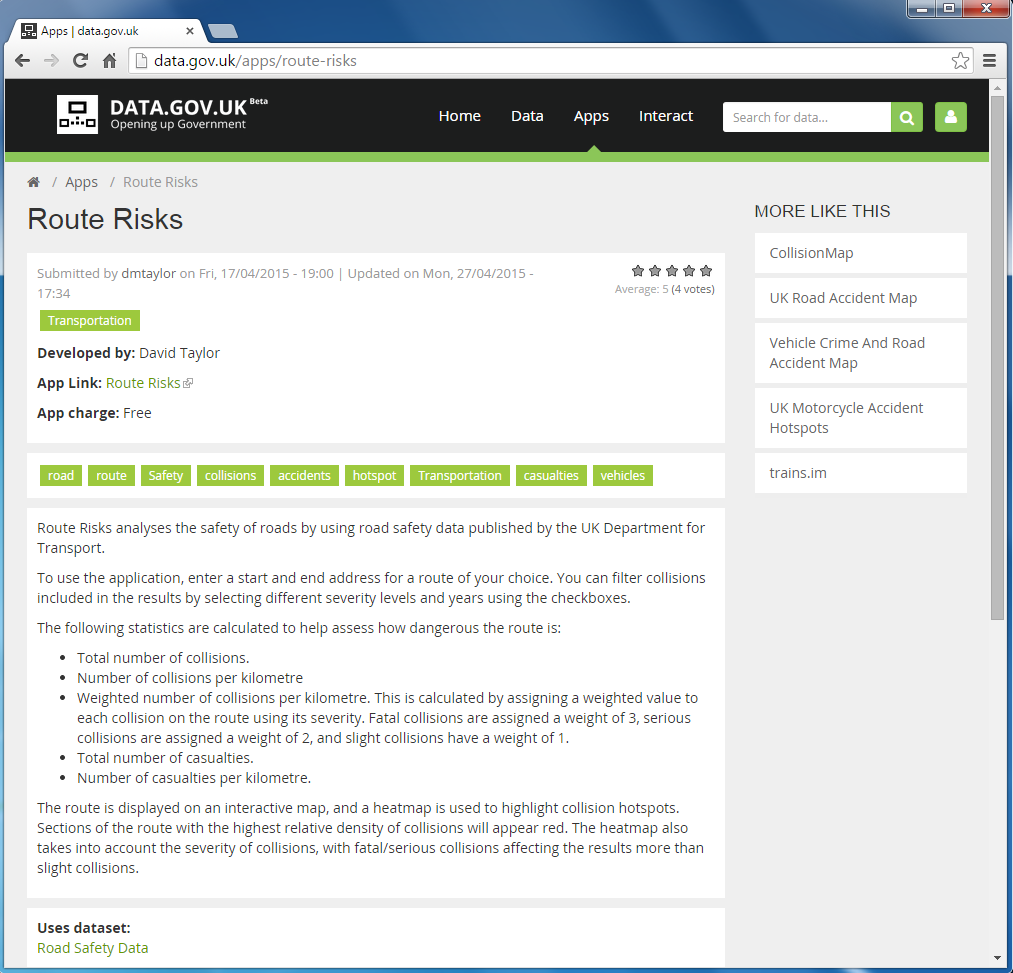
\includegraphics[scale=0.4]{datagovuk}
	\caption{\url{data.gov.uk} page advertising Route Risks}
	\label{fig:datagovuk}
\end{figure}

The technologies used for the application are all open-source, with the exception of the Google Maps API. The application is deployed using a LAMP environment, meaning it uses Linux (Ubuntu), Apache HTTP Server, MySQL and PHP; all of which are open-source. The Google Maps API is free to use for publicly available sites (providing the usage limits are not exceeded), so the only costs associated with the application are for web hosting. The PHP framework used, MINI 1 \citep{mini}, is recommended for projects with low server-side complexity like this, as it is easy to use and set up prototypes in a short period of time. However, more complex projects should look at more advanced frameworks. The Google Maps API is also recommended, as it is free to use, easy to setup, and provides additional libraries with advanced features.

The source code of the application is publicly available on GitHub \citep{Taylor2015}. A link to the repository is included on the website's 'about' page, so that users who are interested in the application will be able to find it. It is envisaged that other developers may use concepts from this project in their own applications.

The agile development methodology used for this project was very useful, and is recommended for similar projects. With the restricted timeframe available, and the unknowns involved with the development process, breaking the project down into increments was essential. This incremental approach ensured that a functional application was delivered.

The project was as expected in terms of complexity and effort required. The main complexity of the project came from filtering the road safety data by route, which was expected as this had not been implemented by other applications. This concept clearly brings great benefits when it comes to analysing the data, and should be used in similar projects. The experience of using Open Data was good, but there was little challenge as only one dataset is used. Potential issues with the quality of the data have been raised, which need to be investigated in future work.

\section{Future Work}

\subsection{Search Accuracy}

When collisions are plotted on the map, many of them appear far away from roads, making it difficult to accurately filter collisions by route. Further investigations should be carried out to find the root cause of this issue. It may be that the accuracy of the latitude and longitude values provided is not sufficient, in which case it is difficult to improve the searching functionality.

However, it should also be considered that there may be an issue with how points are projected onto the map using the Google Maps API. This is unlikely to be the case, as the longitude and latitude values provided are based on the WGS1984 standard \citep{DepartmentforTransporta}, which is the same standard used by the Google Maps API. However, it is a plausible explanation for the issues found, so should not be dismissed without more thorough research and analysis.

\subsection{Safest Route Advice}

The application could be extended to provide more use to general users. For example, some users may wish to find out what the safest route is between two locations. The application could determine this by getting several routes from the Directions Service, and analysing each one before presenting the results to the user.

\subsection{Accessibility}

Accessibility problems with the application should be found and addressed. A known issue involves the use of heatmaps for showing collision hotspots. If a user is colour blind, they may struggle to spot the difference between areas of high and low collision density. This could be solved by letting the user toggle the colour scheme used for the heatmap, or by using other visual aids such as displaying numbers over areas to show how many collisions there are.

\subsection{Automatically Retrieve New Datasets}

When new road safety datasets are released, the current application will not be updated until an administrator downloads the file and manually updates the database. Future effort could be spent on developing a method for automating this process. \textit{Data.gov.uk} provides an API for accessing its data catalogue through both RESTful and functional interfaces \citep{Data.gov.uk}, which would be useful for this. 

\subsection{Other Countries}

The application could be extended to analyse routes in other countries. The complexity in this task would come from integrating multiple datasets from different sources. If the data could be imported into the current data model, the changes to the application would be minimal as the Google Maps API includes mapping and direction services for over 100 countries \citep{Googlea}. Any possible impact on performance would need to be considered before adding more data. It may be necessary to implement caching or pre-computation of popular routes to improve response times.

\subsection{Integration With Other Services}

The application could be integrated with other web services to provide more in-depth analysis. For example, weather services could be used to get a forecast for the specified route at a given time. This data could then be used to analyse the safety of roads in specific weather conditions, as all collisions have weather data associated with them.

\bibliography{library}


\end{document}
